\chapter{休克与循环功能支持}

\section{前沿学术综述}

\subsubsection{休克的概念及其发展过程}

休克是全身有效循环血量明显下降,引起组织器官灌注量急剧减少,导致组织细胞缺氧以及器官功能障碍的临床病理生理过程。有效循环血量明显降低和器官组织低灌注是休克的血流动力学特征,组织缺氧是休克的本质,其最终结果是多器官功能障碍综合征(MODS)。休克的本质决定了休克复苏的根本目标是纠正组织缺氧,防止MODS的发生
\protect\hyperlink{text00008.htmlux5cux23ch1-7}{\textsuperscript{{[}1{]}}}
。

近年来,人们对休克的认识有了不断的提高。对休克认识的进步,实际上反映在对休克发病机制和病理生理的认识进步。休克(shock)的原意为震荡或打击,但直到19世纪,Crile提出休克是震荡或打击引起的以低血压为特征的症候群,才使对休克的认识有了较大的飞跃。

20世纪60年代,Lillehei等通过大量的实验,观察了休克时器官血流量和血流动力学状态,认识到休克是一个以急性微循环障碍为特征的临床综合征,提出了休克的微循环学说。该学说认为休克的本质为有效循环血量减少,导致机体微循环障碍和重要器官灌注不足,引起组织细胞功能紊乱。微循环学说的建立,是历史上对休克进行科学解释的标志。休克时微循环的变化具有一定的规律。根据微循环的改变可将休克分为三个阶段,即微循环缺血期、微循环淤血期和弥散性血管内凝血期。微循环学说从微循环水平科学地解释了休克引起的微循环障碍和器官功能损害,但仍然难以反映休克的本质------有效循环血量减少引起组织缺氧。

组织细胞的缺氧是休克的本质问题。近年来,医学科学的发展使氧代谢及其相关指标的临床应用成为可能。20世纪70年代,血流动力学和氧代谢监测的应用,为休克的血流动力学分类奠定了基础,同时也为观察休克的氧代谢紊乱提供了有力的武器。休克的氧代谢学说是从氧输送和氧消耗以及组织氧需的关系上,探讨休克对全身及器官组织缺氧的影响,是在微循环学说基础上,对休克认识的深化。根据组织缺氧的范围和程度,可将休克分为内脏器官缺氧期和全身器官缺氧期。从组织缺氧的角度去认识休克并指导治疗,是休克认识史上的一大进步。

当休克的微循环障碍、血流动力学紊乱和氧代谢紊乱被纠正后,仍有部分患者发生MODS,包括上消化道出血、急性肾衰竭、弥散性血管内凝血等。也就是说,当休克的微循环障碍、血流动力学和氧代谢紊乱被纠正后,休克仍然可能发展为MODS或多器官功能衰竭。因此,对休克的认识需要进一步深化。20世纪80年代后期,相继发现大量的炎症性细胞因子,炎症反应在休克中的作用也日益受到重视。20世纪90年代,在大量实验和临床研究的基础上,形成了休克的炎症反应和多器官功能障碍学说,该学说的主要内容包括两个方面,首先全身炎症反应可导致休克,即休克是全身炎症反应的后果;其次,休克又可诱发和加重全身炎症反应,导致多器官功能衰竭。

\subsubsection{休克的监测进展}

休克突出表现为血流动力学和氧代谢紊乱。近年来,随着科技的进步,血流动力学和氧代谢的监测取得了迅猛的发展。20世纪80年代,Swan-Ganz肺动脉漂浮导管进入临床,开创了血流动力学监测的新篇章,临床上广泛应用,为休克的治疗提供依据。Swan-Ganz肺动脉漂浮导管监测血流动力学进入临床,使心脏前负荷的监测走向量化,肺动脉嵌顿压和中心静脉压成为反映心脏前负荷的指标。由于肺动脉嵌顿压和中心静脉压受到心脏顺应性、心脏瓣膜功能及胸腔内压力等多种因素的影响,近年大量研究表明,肺动脉嵌顿压和中心静脉压并不能准确反映心脏容量负荷状态
\protect\hyperlink{text00008.htmlux5cux23ch2-7}{\textsuperscript{{[}2{]}}}
\textsuperscript{,}
\protect\hyperlink{text00008.htmlux5cux23ch3-7}{\textsuperscript{{[}3{]}}}
。因此,临床上需要更为可靠的前负荷指标。随着脉搏指示持续心输出量监测技术在临床上的广泛应用,人们可以监测胸腔内血容量、血管外肺水含量及每搏输出量变异度等容量指标来反映机体容量状态,以指导临床容量管理。大量研究证实,胸腔内血容量、每搏输出量变异度、血管外肺水含量可以较准确反映心脏前负荷及肺水肿状态,明显优于肺动脉嵌顿压和中心静脉压等压力指标
\protect\hyperlink{text00008.htmlux5cux23ch4-7}{\textsuperscript{{[}4{]}}}
\textsuperscript{,}
\protect\hyperlink{text00008.htmlux5cux23ch5-7}{\textsuperscript{{[}5{]}}}
。

Swan-Ganz肺动脉漂浮导管和脉搏指示持续心输出量监测均为有创血流动力学监测手段,为了减少创伤,无创性的监测手段应运而生。重复二氧化碳吸入法、阻抗法以及床旁超声均可以进行无创血流动力学监测,并且被证实与有创监测的相关性良好。各种不同方法各有特点,监测指标和利弊各有不同,临床上可根据患者情况选择合适的监测手段
\protect\hyperlink{text00008.htmlux5cux23ch6-7}{\textsuperscript{{[}6{]}}}
\textsuperscript{~}
\protect\hyperlink{text00008.htmlux5cux23ch8-7}{\textsuperscript{{[}8{]}}}
。

\subsubsection{休克的治疗现状}

基于对休克认识和监测水平的提高,休克的血流动力学支持和治疗也有了长足的进步。血管活性药物使用不仅仅是为了改善血流动力学状态,更重要的是改善组织的灌注,从而达到改善预后的目的。

严重感染和感染性休克是以全身性感染导致器官功能损害为特征的复杂的临床综合征,目前病死率仍高达30%~70%。面对严重感染和感染性休克的挑战,2002年10月欧洲危重病医学会、美国危重病医学会和国际感染论坛在西班牙巴塞罗那共同发起了拯救全身性感染的全球性行动倡议------拯救全身性感染运动(surviving
sepsis
campaign),并且在2004年扩大到11个学会共同制定《重症感染和感染性休克治疗指南》(简称《指南》),旨在规范临床治疗,最终降低严重感染和感染性休克病死率
\protect\hyperlink{text00008.htmlux5cux23ch9-7}{\textsuperscript{{[}9{]}}}
,该《指南》并在2008及2012年进行了更新。但有研究证实,该《指南》的依从性较差。为了进一步落实该《指南》在临床的应用,《指南》从中提炼出明确降低病死率的核心的几项内容,形成一个联合治疗的套餐,称之为“感染的集束化治疗”(sepsis
bundle),一方面为了促进临床医生联合应用集束化治疗的各项措施,另一方面也是为了简化,利于临床医生操作,提高依从性和可行性,从而规范临床严重感染及感染性休克的治疗行为,最后达到降低病死率的目的
\protect\hyperlink{text00008.htmlux5cux23ch10-7}{\textsuperscript{{[}10{]}}}
\textsuperscript{,}
\protect\hyperlink{text00008.htmlux5cux23ch11-7}{\textsuperscript{{[}11{]}}}
。

感染的集束化治疗指在确诊严重感染立即开始并在6小时内必须完成的治疗措施,包括:①血清乳酸水平测定;②抗生素使用前留取病原学标本;③急诊在3小时内,重症医学科在1小时内开始广谱抗生素治疗;④如果有低血压或血乳酸>4mmol/L,立即给予液体复苏(20ml/kg),如低血压不能纠正,加用血管活性药物,维持平均动脉血压>65mmHg(1mmHg=0.133kPa);⑤持续低血压或血乳酸>4mmol/L,液体复苏使中心静脉压>8mmHg,中心静脉血氧饱和度>70%。

Levy等研究表明,随着《指南》的简化和推广,临床医生对其依从性有了明显的提高(从10.9%提高至31.3%),随着依从性的提高,患者的病死率得到明显的下降。然而,目前6小时感染的集束化治疗达标率仍然不足1/3,而在中国,其达标率甚至不到10%,因此需要继续针对临床医生进行教育及培训,以提高《指南》的依从性,进而降低严重感染和感染性休克的病死率。

近年来,循环功能的机械辅助取得了长足的进步。目前临床上应用最广泛的循环辅助装置是主动脉内球囊反搏,但对严重的左心室衰竭,可考虑应用左心室辅助,严重的双心室衰竭可考虑双室辅助、人工心脏等。对急性心功能障碍、心肌损害的患者,如心脏手术后低心排综合征、急性大面积心肌梗死、心源性休克、急性心肌炎、心功能障碍和急性移植心脏衰竭等,应用心室辅助装置的目的是减少心脏做功,维持和改善全身循环,促进心肌损伤修复。心室辅助装置的置入在改善全身器官循环灌注的同时,也为心肌损伤的修复提供了时间和条件,部分病人可能在心脏功能恢复后撤离机械循环支持。国内主动脉内球囊反搏的使用在许多重症医学科已经具有丰富的临床经验,但心室辅助和人工心脏还正在起步中。

\section{临床问题}

\subsection{休克的相关概念和发病机制}

\subsubsection{怎样认识休克的概念和本质?}

休克是各种原因导致的全身有效循环血量明显下降,引起组织器官灌注量急剧减少,导致组织细胞缺氧以及器官功能障碍的临床病理生理过程。有效循环血量明显降低和器官组织低灌注是休克的血流动力学特征,组织缺氧是休克的本质,其最终结果是多器官功能障碍综合征。严格来说,休克是多种原因引起的、具有相同或相似临床表现的一组临床综合征。

\subsubsection{休克一定有低血压吗?}

血压降低是休克最常见、最重要的临床特征,但将血压降低作为是否发生休克的分水岭,显然是错误的。休克早期,以器官低灌注状态为主要表现,患者可出现心动过速、皮肤及四肢湿冷、少尿等,但血压并不一定降低,有时甚至升高。原有高血压者,发生休克时血压可能仍处于正常范围。另外,全身低灌注状态的患者,外周动脉血压测量值往往高于中心动脉血压,外周动脉压并不能反映器官灌注情况。因此,休克并不一定要伴有低血压,即使血压不低,也可能已发生休克,而一旦出现低血压,则表明已经进入休克的失代偿期。可见,在休克的诊断和治疗中,血压是一个非常重要的指标,但不敏感,以血压降低作为诊断休克的标准显然是片面的。

\subsubsection{休克发生的基本环节是什么?}

尽管休克的病因复杂,但有效循环血量减少导致组织器官有效灌注减少是休克发生的共同基础。器官有效灌注的实现依赖于足够的血容量、正常的血管容积(正常的血管收缩和舒张功能)及正常的心脏泵功能。任何一个环节障碍,都会影响器官的有效灌注,导致休克。

(1)血容量减少 血容量减少导致静脉回流减少,心脏充盈不足,心输出量降低,进而引起血压下降。另外,交感神经兴奋,导致外周血管痉挛,也导致组织器官灌注减少。

(2)血管容量增加 血管床的容积很大,正常毛细血管是交替开放的,多数处于关闭状态,毛细血管内的血量仅占总血容量的6%。如毛细血管均开放,则仅肝脏毛细血管就可容纳全身的血容量。因此,毛细血管正常的交替性开放状态是维持有效循环血量的重要环节。休克时,由于组织缺氧、酸中毒以及一氧化氮等扩血管介质的大量释放,导致毛细血管床扩张,血管容量明显增加,导致有效循环血量降低,最终器官有效灌注明显减少。

(3)心脏泵功能障碍 各种原因导致的心脏泵功能障碍,均使心输出量降低,引起血压降低,器官有效灌注明显减少。

\subsubsection{休克发生的病理生理机制有哪些?}

对休克认识的进步,实际上反映了对休克发病机制和病理生理的认识进步。目前,对于休克发病的病理生理机制包括3个学说:休克的微循环学说、休克的氧代谢学说和休克的炎症反应和多器官功能障碍学说。

(1)休克的微循环学说 20世纪60年代,Lillehei等通过大量的实验观察了休克时器官血流量和血流动力学状态,认识到休克是一个以急性微循环障碍为特征的临床综合征,提出了休克的微循环学说。休克时微循环的变化具有一定的规律。根据微循环的改变可将休克分为3个阶段,即微循环缺血期、微循环淤血期和弥散性血管内凝血期。

(2)休克的氧代谢学说 组织细胞的缺氧是休克的本质问题。休克的氧代谢学说是从氧输送和氧消耗以及组织氧需的关系上,探讨休克对全身及组织缺氧的影响,是在微循环学说基础上,对休克认识的深化。根据休克的发展过程,可将休克分为内脏器官缺氧期和全身器官缺氧期。

(3)休克的炎症反应和多器官功能障碍学说 20世纪80年代后期,炎症性细胞因子相继发现,炎症反应在休克中的作用也日益受到重视。20世纪90年代,在大量实验和临床研究的基础上,形成了休克的炎症反应和多器官功能障碍学说,该学说的主要内容包括两个方面,首先全身炎症反应可导致休克,即休克是全身炎症反应的后果;其次,休克又可诱发和加重全身炎症反应,导致多器官功能衰竭。

\subsection{休克的分类和临床特征}

\subsubsection{如何对休克进行分类?}

休克的分类临床上常有病因分类和血流动力学分类。病因分类是基础,血流动力学分类是病因分类的必要补充,反映了休克的诊断和治疗是以纠正血流动力学紊乱和氧代谢障碍为目标。

(1)病因分类 病因分类以导致休克的基础疾病或原因进行分类,有助于诊断基础疾病、及时消除病因。从另一个侧面,也反映出对休克认识的局限性。

低血容量性休克:失血性休克(急性消化道出血、肝脾破裂、宫外孕及产科出血等);创伤性休克(严重创伤、骨折、挤压伤、大手术及多发性损伤等);烧伤性休克(烧伤引起大量血浆丢失);失液性休克(大量呕吐、腹泻、出汗、肠瘘等)。

感染性休克:常见于肺炎、急性化脓性胆管炎、急性肠梗阻、胃肠穿孔、急性弥漫性腹膜炎、中毒性菌痢等疾病。

心源性休克:常见于急性心肌梗死、心律失常、心包填塞、心脏手术后、重症心肌炎、感染引起的心肌抑制等。

过敏性休克:常见于药物(如青霉素)、血清制剂、输血或血浆等引起的过敏反应,蚊虫、蜜蜂等叮咬过敏,花粉、化学气体过敏等。

神经源性休克:常见于高度紧张、恐惧、高位脊髓损伤、脊髓神经炎、脑疝、颅内高压等。

内分泌性休克:常见于肾上腺皮质功能不全或衰竭、糖皮质激素依赖等。

(2)血流动力学分类 随着对休克认识的进步和治疗手段更新,尤其是血流动力学监测应用于临床后,休克患者死亡的主要原因不再是基础疾病,而是由此造成的循环功能及其他器官功能障碍。原有的休克病因分类方法就显得明显不足。同时,不同病因导致的休克可表现为相同或相近的血流动力学改变。可以依据血流动力学特点来指导休克的治疗,因此对休克进行血流动力学分类就显得很有必要。按血流动力学的变化,可将休克分为低血容量休克、心源性休克、分布性休克和梗阻性休克。

\subsubsection{按血流动力学分类,各类休克的特点是什么?}

低血容量休克的基本机制是循环容量丢失,大量体液丧失使血容量急剧减少,心脏前负荷不足,导致心输出量下降,氧输送和组织灌注明显减少。血流动力学特点为中心静脉压下降、肺动脉嵌顿压下降、心输出量减少、心率加快和体循环阻力增高。

心源性休克的基本机制为泵功能衰竭,指在保证足够前负荷的条件下,心输出量明显下降。心输出量、搏功指数、左心室射血分数、左心室舒张末期压力及容积等均是反映心脏泵功能的重要指标,监测这些指标有助于明确泵功能衰竭的原因。血流动力学特征是心脏泵功能衰竭导致心输出量急剧下降,中心静脉压升高,肺动脉嵌顿压升高,体循环阻力升高。

分布性休克的基本机制为血管收缩舒张功能调节异常。这类休克中,一部分表现为体循环阻力正常或增高,主要是容量血管扩张,循环血量相对不足所致。常见原因包括神经节阻断、脊髓休克等神经性损伤或麻醉药物过量等,另一部分是以体循环阻力降低为主要表现,导致血液重新分布,主要见于感染性休克。严重的全身炎症反应也可引起分布性休克,主要见于重症急性胰腺炎早期、严重烧伤早期等。典型的血流动力学特点是心输出量升高或正常,伴体循环阻力降低。低血压、脉搏洪大、四肢末梢温暖是常见的临床特征。当然,当感染性休克合并心源性或低血容量因素时,症状与体征往往不典型。感染性休克时的心功能改变表现为心血管功能抑制,包括心脏收缩功能和舒张功能异常以及血管张力和血流异常。

梗阻性休克的基本机制是血流通道受阻,如腔静脉梗阻、心包缩窄或填塞、心瓣膜狭窄、肺动脉栓塞等。由于血流通道受阻导致心输出量减少,引起循环灌注不良。心输出量减少导致氧输送降低、组织缺血缺氧是梗阻性休克的共同特征。

\subsubsection{休克的早期诊断应注意什么?}

休克的诊断至少应包括几方面的内容:休克的病因、伴或不伴血压下降,组织灌注不足及组织缺氧的表现,器官功能的改变。

准确地说,休克是多种原因引起的具有相同或相似临床表现的一组临床综合征。当致病因素作用于机体后,休克的病理生理过程已经开始,但临床上并不会立即表现出血压下降或其他反映休克的临床指标,甚至休克的病理生理过程已经发展一段时间后,临床表现也不典型。因此,休克的发生发展是一个连续的病理生理过程,诊断治疗应当强调“早”。

休克的诊断一般不难,关键是应早期及时发现。要点是凡遇到严重损伤、大出血、严重感染以及过敏的病人和有心脏病史者,应想到发生休克的可能;如出现出汗、兴奋、心率加快、脉压差小或尿少等症状者,应疑有休克。若病人出现神志淡漠、反应迟钝、皮肤苍白、呼吸浅快、收缩压降至90mmHg,或原有高血压的患者收缩压下降40mmHg及尿少者,则标志患者已进入休克失代偿期。

\subsubsection{重视严重感染的临床意义是什么?}

感染是指无菌的体液或体腔中发现微生物,全身性感染是指这些微生物的侵入导致机体出现全身炎症反应,也就是合并全身炎症反应综合征的发生。当全身性感染并发器官功能损害时,称为严重感染。感染性休克是严重感染的特殊形式。当严重感染合并循环功能衰竭时,称为感染性休克。

严重感染和感染性休克是以全身性感染导致器官功能损害为特征的复杂临床综合征,其发病率和病死率均很高。全世界每年大约1000人中就有3人发生严重感染和感染性休克,同时这一数字还呈现不断增长的趋势。近年来,抗感染治疗和器官功能支持技术取得了长足的进步,临床医师对《指南》的依从性也明显提高,但严重感染的病死率仍高达30%以上。在美国,严重感染是第10位的致死原因,其死亡人数超过乳腺癌、直肠癌、结肠癌、胰腺癌和前列腺癌致死人数的总和。因此,必须高度重视严重感染和感染性休克的严峻形势,并不断探索规范的诊断方法和有效的治疗手段。

\subsubsection{感染性休克的诊断标准是什么?}

临床上感染性休克诊断需符合以下标准:①有明确感染灶;②有全身炎症反应存在;③收缩压低于90mmHg,或较原来基础值下降40mmHg,经液体复苏后1小时不能恢复或需血管活性药维持;④伴有器官组织的低灌注,如尿量<30ml/小时,或有急性意识障碍等;⑤血培养可能有致病微生物生长。

当临床上存在严重感染伴有发热或体温不升、意识障碍、过度通气、皮肤潮红、脉搏洪大等临床表现时,感染性休克容易诊断。但临床表现不典型时,易漏诊或误诊。年老体弱和免疫功能低下的患者往往缺乏典型的临床表现。另外,感染性休克患者存在心功能不全及血容量不足时,同样表现为皮肤湿冷及脉搏细速,与心源性休克及低血容量休克不易鉴别。意识障碍及少尿对感染性休克的诊断并不特异。

\subsubsection{高排低阻的感染性休克患者,其心脏功能是正常的吗?}

典型的感染性休克血流动力学特点是心输出量升高或正常,伴体循环阻力降低。但心输出量的增加或正常不代表感染性休克患者心功能正常。相反,感染性休克时的心功能改变表现为心血管功能抑制,包括心脏收缩功能和舒张功能异常。

(1)心肌收缩力降低 在左室压力容积环中,左室等容收缩曲线的斜率明显降低,说明左室收缩力显著降低(图\ref{fig2-1}),其机制与心肌抑制因子及肿瘤坏死因子等对心肌的直接抑制效应有关,也与血压降低导致心肌灌注减少和缺氧有关。另外,感染导致心脏毛细血管内皮细胞损伤和白细胞激活,白细胞在毛细血管内聚集,堵塞毛细血管,加重心肌缺血,也与心肌收缩力降低有关。心肌收缩力的下降随着患者的康复,5~10天后可以逆转。

\begin{figure}[!htbp]
 \centering
 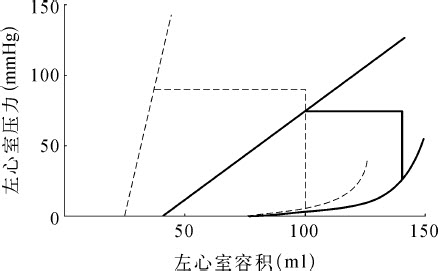
\includegraphics{./images/Image00010.jpg}
 \captionsetup{justification=centering}
 \caption{感染性休克时左心室压力容积的变化(虚线为正常心功能,实线为感染性休克)}
 \label{fig2-1}
  \end{figure} 



(2)心肌顺应性代偿性改变 感染性休克时,多数患者心肌顺应性明显增加,但也有部分患者心肌顺应性降低。

心肌顺应性增加伴心输出量增加:感染性休克时,心室代偿性扩张,则心肌顺应性明显改善,左室舒张期顺应性曲线向右下移位,左室舒张末期容积明显增加,使每搏输出量增加,心功能曲线上表现为曲线向左上方向移位(图\ref{fig2-2})。

\begin{figure}[!htbp]
 \centering
 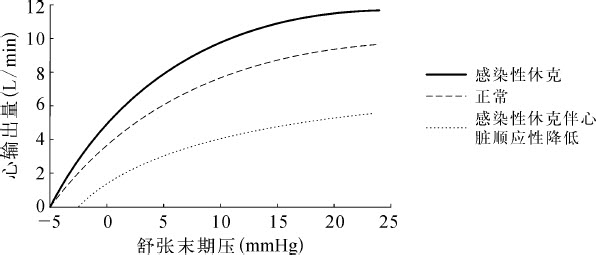
\includegraphics{./images/Image00011.jpg}
 \captionsetup{justification=centering}
 \caption{感染性休克时心功能曲线的改变}
 \label{fig2-2}
  \end{figure} 

心肌顺应性降低伴心输出量降低:若心室未发生代偿性扩张,甚至左室顺应性明显降低,则左室压力容积曲线就表现为舒张期顺应性曲线向左上移位,左室舒张末期容积降低,加之心室等容收缩曲线向右下移位,使左室收缩末期容积增加,结果每搏输出量明显降低,使心输出量明显减少。心功能曲线上则表现为曲线向右下移位(图\ref{fig2-2})。部分患者心室不能发生代偿性扩张的机制尚不清楚,推测可能与内源性儿茶酚胺大量释放、外源性大剂量儿茶酚胺类和洋地黄类药物应用有关,导致心肌纤维过度收缩,心室过度排空,引起心肌舒张受限,使心肌顺应性显著降低。研究显示,左室不能代偿性舒张、顺应性明显降低的感染性休克患者,病死率明显升高。

值得注意的是,心肌细胞水平(心肌细胞收缩力-心肌纤维初长度)和心脏整体水平(心输出量-左室舒张末期容积)的心功能曲线可能是不一致的。感染性休克时,心肌细胞水平上的心功能曲线均向右下移位,表现为心肌细胞收缩力明显降低。但在整体心脏水平上,心功能曲线体现左室前负荷与心输出量或左室搏功指数的关系,曲线的走向不仅受心肌收缩力的影响,还受心室顺应性以及后负荷的影响。当左室顺应性明显改善、后负荷明显降低时,心输出量明显增加,多数感染性休克患者表现为心输出量明显增加。整体水平的心功能曲线就表现为曲线向左上移位,与心肌细胞水平的心功能曲线改变方向相反。当然,当左室顺应性降低时,即使后负荷降低或不变,心输出量也呈现明显降低,其结果是心脏整体水平的心功能曲线向右下移位,与心肌水平上心功能曲线的改变趋势一致。

\subsubsection{哪些原因可以导致心源性休克?}

心源性休克是由于急性心泵功能衰竭或严重心律紊乱(心室纤维震颤等)而导致的休克。心输出量、心脏做功指数、左心室射血分数、左心室舒张末期压力及容积等均是反映心脏泵功能的重要指标,监测这些指标有助于明确泵功能衰竭的原因。

心源性休克可由心脏收缩功能降低、舒张功能障碍(包括顺应性下降)、心律失常等原因引起(表\ref{tab2-1})。心瓣膜狭窄、心室流出道梗阻等心内梗阻性的原因造成的心输出量下降,其本质上并不是泵功能衰竭,治疗上也与泵功能衰竭明显不同。因此,心内梗阻引起的休克已经不再被认为是心源性休克,应该属于梗阻性休克。

\begin{table}[htbp]
\centering
\caption{心源性休克的常见原因}
\label{tab2-1}
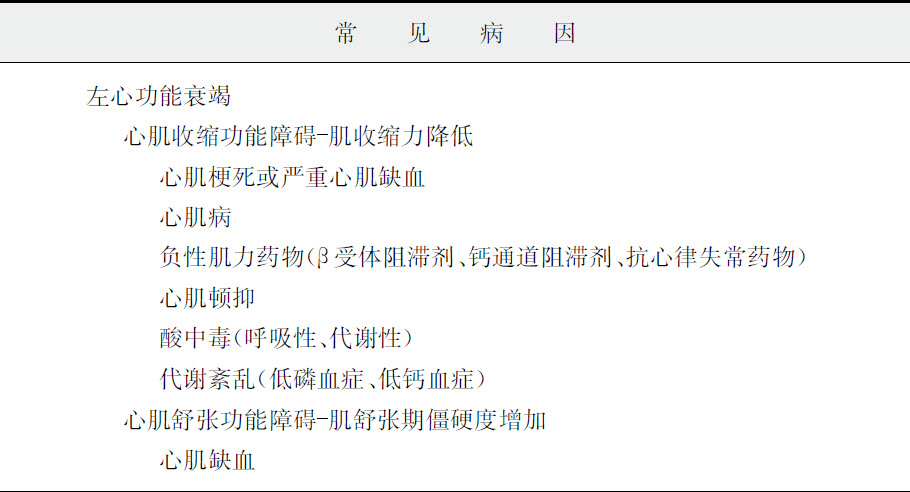
\includegraphics[width=\textwidth,height=\textheight,keepaspectratio]{./images/Image00012.jpg}
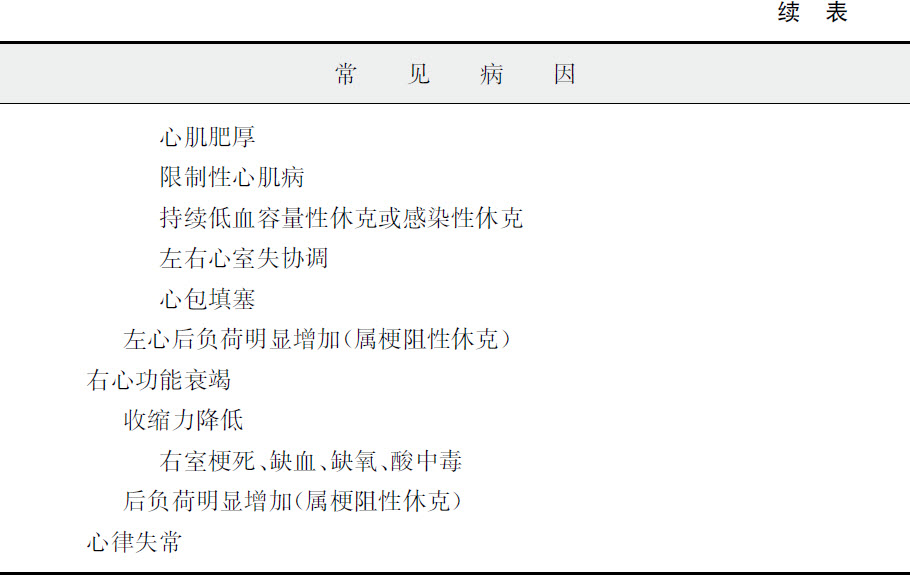
\includegraphics[width=\textwidth,height=\textheight,keepaspectratio]{./images/Image00013.jpg}
\end{table}



\subsubsection{如何认识心脏舒张功能障碍在心源性休克中的地位?}

发生心源性休克时,心脏收缩功能和舒张功能障碍均有障碍,但临床上心室舒张功能障碍往往被忽视,从而导致治疗失败。

心室舒张功能障碍引起心源性休克时,多表现为心输出量降低,心室充盈压力明显升高。床边经食管超声心动图检查若显示心室舒张末期容积减小,射血分数较高,则可证实心室顺应性降低。另外,液体负荷试验也有助于了解心室顺应性,采用5%葡萄糖溶液或生理盐水50~100ml在5~10分钟内快速静脉输注,比较输液前后中心静脉压或肺动脉嵌顿压的改变。如果压力无明显增加或增加幅度较小,提示患者心室顺应性较好;输液后压力明显增加,则提示顺应性较差。

心输出量呈现心率依赖性,也提示心室舒张期充盈障碍、顺应性降低。心率过快、过慢均影响心室舒张期充盈。心脏顺应性降低时,较少的心室充盈即可使心室舒张压力明显增加,此时,心率的增加可使心输出量明显增加。

心肌缺血引起的顺应性降低,若能及时去除病因,心室顺应性可明显改善。但一般情况下,改善心肌顺应性很困难。应用正性肌力药可使收缩力增加,但顺应性可能进一步降低。硝酸酯类扩血管药物降低心脏后负荷的同时,也可改善心肌顺应性,是改善心肌顺应性的重要治疗措施之一。若心室顺应性不能改善,患者可能因后负荷下降而出现血压下降。因此,舒张功能障碍在心源性休克中的作用值得重视。传统的心源性休克治疗集中于改善心脏收缩功能,显然是不合适的。

\subsubsection{怎样诊断心源性休克?}

心源性休克的临床诊断必须满足两个条件:一是有休克的临床表现,二是存在心脏的疾病。心源性休克的临床表现和其他类型的休克是类似的。

总的来说,早期患者烦躁不安、焦虑、面色苍白、肢体冰冷、皮肤呈花纹状、出冷汗、周围型紫绀、心率快、血压低、尿量明显减少。如果患者有严重的左心功能不全,可出现急性肺水肿表现,如胸闷气促、咯粉红色泡沫样血痰、两肺满布湿啰音。如果是心脏瓣膜的腱索断裂或是心肌梗死后室间隔穿孔,可以听到心脏杂音。在心源性休克的晚期,可以出现DIC而发生全身皮肤、黏膜和内脏广泛出血,并出现多器官功能障碍或衰竭,此时治疗已十分困难。

辅助检查有助于心源性休克的诊断。

(1)心电图 应对患者做12导联的心电图描记(必要时做18导联),对各种心律失常、电解质紊乱、心肌供血不足和心肌梗死(包括病变范围)等,可获得重要的数据资料。

(2)床边X线片检查 可了解两肺情况,胸腔有无积液、积气,心脏大小和纵隔有无增宽等情况。

(3)动脉血气分析 可了解患者呼吸功能情况和有无酸碱平衡失调,有无水电解质代谢紊乱。

(4)动脉压监测 建议对休克患者应用有创的动脉内连续测压方法监测血压,观察整个病情过程中血压的动态变化。

(5)血流动力学监测 置入Swan-Ganz肺动脉漂浮导管,可监测较全面的血流动力学指标,如中心静脉压、肺动脉压、肺动脉嵌顿压,并可测定心输出量。

(6)血液生化检查 心肌酶谱的测定、肝肾功能的测定、凝血酶原时间和部分凝血活酶时间及有关DIC的检查如3P试验,可以了解其他器官的功能状态和病情的进展。

\subsubsection{休克不同阶段的临床特点是什么?}

不同类型的休克,其临床过程有不同的特点。根据休克的病程演变,休克可分为两个阶段,即休克代偿期和休克抑制期,或称休克前期和休克期。

(1)休克代偿期 有效循环血量降低20%以下时,由于机体的代偿作用,患者的中枢神经系统兴奋性提高,交感神经活动增加,表现为精神紧张或烦躁、面色苍白、手足湿冷、心率加速、过度换气等。血压正常或稍高,反映小动脉收缩情况的舒张压升高,故脉压缩小。尿量正常或减少。这时,如果及时处理,休克可以很快得到纠正。如果处理不当,则病情发展,进入抑制期。

(2)休克抑制期 有效循环血量降低20%以上或处于失代偿期的休克迟迟得不到纠正,则进入休克抑制期。患者神志淡漠、反应迟钝,甚至可出现神志不清或昏迷、口唇肢端发绀、出冷汗、脉搏细速、血压下降、脉压差显著缩小。严重时,全身皮肤黏膜明显紫绀,四肢冰冷,脉搏扪不清,血压测不出,无尿。皮肤、黏膜出现淤斑或消化道出血,提示合并DIC。

并发其他器官功能障碍,如患者出现进行性呼吸困难、脉速、烦躁、紫绀或咯出粉红色痰,动脉血氧分压降至60mmHg以下,吸氧也不能提高动脉氧分压和改善症状时,常提示发生急性呼吸窘迫综合征。

休克的临床表现一般都随休克的病程演变而改变(表\ref{tab2-2})。

\begin{table}[htbp]
\centering
\caption{休克代偿期和抑制期的临床特征}
\label{tab2-2}
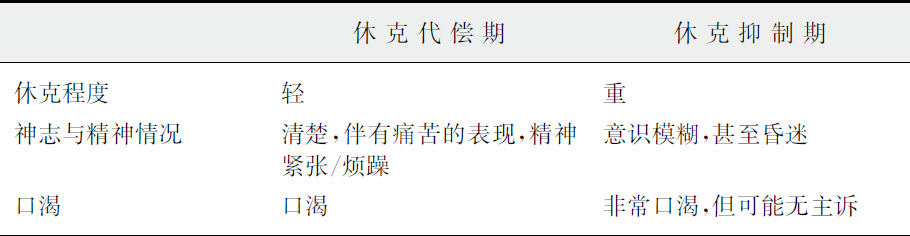
\includegraphics[width=\textwidth,height=\textheight,keepaspectratio]{./images/Image00014.jpg}
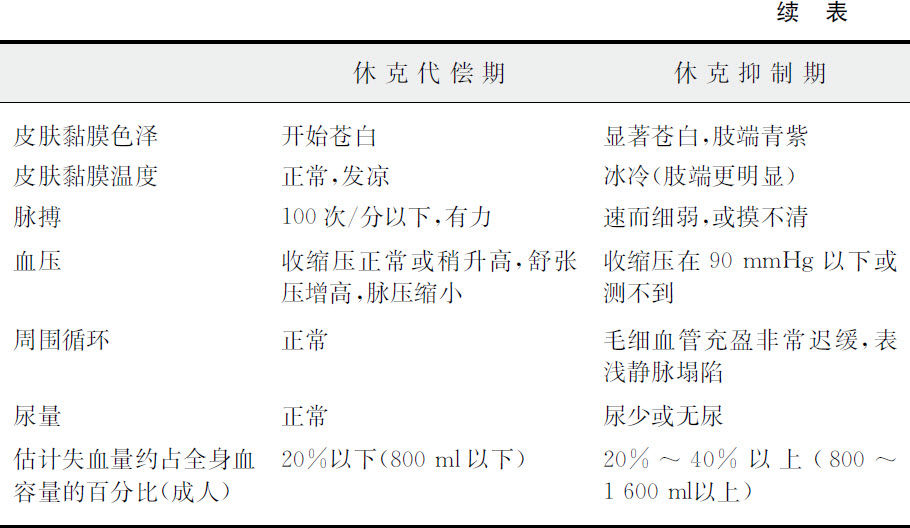
\includegraphics[width=\textwidth,height=\textheight,keepaspectratio]{./images/Image00015.jpg}
\end{table}



\subsection{休克的监测}

\subsubsection{对休克患者临床观察的基本要点有哪些?}

(1)意识状态 能够反映脑组织的灌注情况。患者神志清楚,反应良好,表示循环血量已够;神志淡漠或烦躁、头昏、眼花,或从卧位改为坐位时出现晕厥,则常表示有效循环血量不足。

(2)肢体温度和色泽 反映末梢灌注情况。患者四肢温暖,皮肤干燥,轻压指甲或口唇时,局部暂时缺血呈苍白,松压后迅速转红润,表明休克好转;四肢皮肤常苍白、湿冷,轻压指甲或口唇时颜色苍白,在松压后恢复红润缓慢,表明休克未纠正。

(3)血压 休克代偿期,剧烈的血管收缩,血压可以保持或高于正常;休克抑制期血压逐渐下降,收缩压低于90mmHg,脉压低于20mmHg;血压回升,脉压增加,则表明休克有所好转。

(4)心率或脉率 心率加快或脉率细速常常出现在血压下降之前。有时血压仍低,但脉搏清楚、手足温暖,则提示休克趋于好转。休克指数[脉率/收缩期血压(以mmHg表示)]有助于判断休克的程度。休克指数正常为0.5,表示无休克;超过1.0~1.5表示存在休克;在2.0以上,则表示休克严重。

(5)尿量 尿量是反映肾脏灌注情况的指标,也可反映器官血流灌注情况。休克患者应常规放置导尿管,观察每小时尿量和尿比重。尿量少于25ml/小时、尿比重增加,说明肾血管收缩或血容量仍不足;血压正常,但尿量仍少,尿比重高,反映肾脏灌注仍然不足;如血压正常,尿量少,尿比重低,则可能发生急性肾衰竭。尿量稳定在每小时30ml以上时,表示休克好转。

\subsubsection{怎样评价中心静脉压监测在休克中的作用?}

当一般临床观察难判断休克患者血容量状态时,可考虑通过放置颈内静脉导管或锁骨下静脉导管监测中心静脉压,也可通过Swan-Ganz肺动脉漂浮导管监测中心静脉压。

中心静脉压是反映患者血容量状态的指标,正常值为5~10cmH\textsubscript{2}
O。一般认为,中心静脉压<5cm H\textsubscript{2}
O提示血容量不足;中心静脉压>15cm H\textsubscript{2}
O提示输液过多或心功能不全。然而,对于重症患者,中心静脉压的绝对值并不能准确反映容量状态。有研究分析中心静脉压绝对值与血容量的相关性,显示其相关性仅为0.16。

连续、动态监测中心静脉压可能更具有临床意义。通过容量负荷试验,观察中心静脉压的改变,有助于评价患者的容量及心功能状态。然而,也有研究同样证实中心静脉压的变化值不能有效预测容量反应性。

\subsubsection{如何评价肺动脉嵌顿压在休克中的作用?}

肺动脉嵌顿压(PAWP)可通过Swan-Ganz肺动脉漂浮导管监测,是反映左心室前负荷水平的指标,正常值为8~15mmHg。与中心静脉压相比,能够更准确地反映机体容量状态。一般认为,肺动脉嵌顿压<6mmHg提示容量严重不足;肺动脉嵌顿压<12mmHg仍提示容量不足;肺动脉嵌顿压12~15mmHg提示容量正常或容量不足伴左心功能不全;肺动脉嵌顿压>15mmHg提示容量过多或伴左心功能不全,有发生肺水肿的危险性。

然而,同中心静脉压一样,对于重症患者,肺动脉嵌顿压的绝对值也不能有效预测患者的容量反应性,而动态观察肺动脉嵌顿压的改变具有更高价值。

\subsubsection{全身氧代谢监测主要包括哪些指标?}

全身氧代谢监测主要包括氧输送、氧耗量、氧摄取率及混合静脉血氧分压或饱和度等监测指标。

(1)氧输送 指单位时间内心脏泵血所提供给组织细胞的氧量,由呼吸功能(动脉血氧饱和度和氧分压)、血液系统功能(血红蛋白浓度)和心脏泵功能(心指数)3个因素决定。氧输送正常值为每分钟500~600ml/m\textsuperscript{2}
。

(2)氧耗量 是单位时间内组织器官所消耗的氧量。正常值为每分钟160~220ml/m\textsuperscript{2}
。感染性休克时氧耗量常常与氧输送具有病理依赖关系,即随氧输送增加,氧耗量也明显增加。

(3)氧摄取率 单位时间内组织的氧耗量占氧输送的比例。正常值为20%~30%。计算公式:氧摄取率=氧耗量/氧输送。

(4)氧需(oxygen
demand) 为单位时间内维持组织细胞正常代谢所需消耗的氧量。根据Shoemaker方法,氧需可经麻醉和体温校正后估算。氧需=氧耗量(麻醉)×10-0.036667×(98.6-T),其中T为华氏温度,氧耗量(麻醉)=10×体重(kg)×0.72。

(5)氧债(oxygen
debt) 反映机体缺氧的程度。根据氧需与机体实际氧耗量的关系,就可判断机体是否缺氧。当氧耗量与氧需的差值大于零时,说明机体不缺氧,无氧债。但当氧耗量与氧需的差值小于零时,则组织存在氧债,提示组织缺氧。因此,组织是否缺氧决定于氧供与氧需是否能够保持平衡。

(6)动脉血pH值 正常值7.35~7.45。低于7.35提示存在酸中毒。

(7)血乳酸浓度 正常值1~1.5mmol/L。休克时间越长,组织器官低灌注越严重,动脉血乳酸浓度越高。乳酸浓度持续升高,表示病情严重,预后不佳。

(8)混合静脉血氧饱和度或氧分压 正常值分别为>65%和>40mmHg。

\subsubsection{什么是胃肠黏膜pH值,如何监测?}

监测血流动力学及氧输送仅能了解全身氧代谢,难以反映内脏器官的氧代谢。但是,缺氧最早发生在组织细胞水平,监测器官组织水平的血流灌注和氧代谢,具有特别重要的意义。20世纪80年代出现的监测胃肠黏膜pH值的方法,是目前唯一应用于临床、直接监测胃肠道黏膜灌注及氧代谢的技术。

pHi是通过特殊的导管间接测量胃肠腔内的二氧化碳分压和动脉血的碳酸氢根浓度来完成的。1982年Fiddian-Green提出,在一定条件下,将张力法测得的胃肠黏膜二氧化碳分压和同步测量的动脉血碳酸氢盐浓度(\ce{HCO3-}
),代入改良的Henderson-Hasselbalch公式,可计算出胃肠黏膜pH值(pHi):$\text{pHi}=6.1+1\text{g} (\ce{HCO3-}/\text{PrCO}_2\times 0.03\times k)$
,公式中0.03为二氧化碳的解离常数,k为不同平衡时间相对应的校正系数,PrCO\textsubscript{2}
为胃肠黏膜二氧化碳分压。pHi计算必须满足的3个假设:①二氧化碳能在组织间自由弥散;②胃肠腔内液体中的二氧化碳分压等于黏膜内二氧化碳分压;③动脉血中的碳酸氢盐浓度与胃肠黏膜中的碳酸氢盐浓度相等。

\subsubsection{目前常用的器官氧代谢的监测手段有哪些?}

系统监测机体的氧代谢状况,需从全身、器官及细胞3个层次进行(表\ref{tab2-3}),但是床边危重患者的细胞水平氧代谢监测仍困难。当前主要通过监测机体氧输送有关指标、血乳酸浓度及器官功能来评价机体氧代谢状况,目前常用的器官的氧代谢监测手段如下。

\begin{table}[htbp]
\centering
\caption{机体氧代谢的监测指标}
\label{tab2-3}
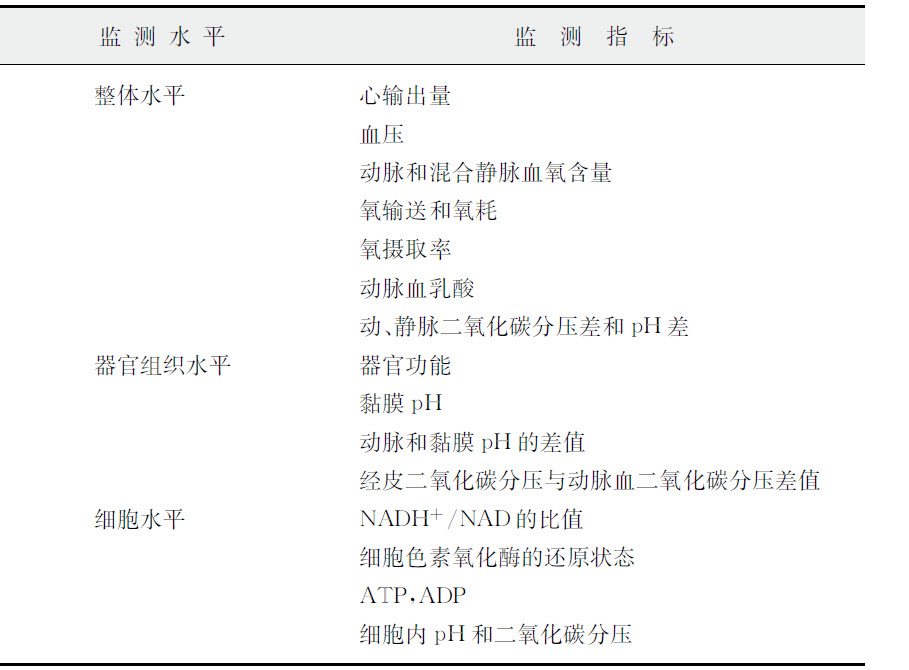
\includegraphics[width=\textwidth,height=\textheight,keepaspectratio]{./images/Image00019.jpg}
\end{table}

(1)胃黏膜pH值 胃黏膜pH值反映胃肠道黏膜的灌注和代谢情况,是反映休克引起胃肠道低灌注的敏感指标。休克时,肠道是最早缺血缺氧的器官,而休克纠正时,肠道又是灌注恢复最晚的器官。通过特殊的胃黏膜氧张力计监测胃黏膜pH值。正常值为7.35~7.45。胃黏膜pH值<7.35说明胃肠道缺血缺氧,胃黏膜pH值水平越低,说明胃肠道缺血越严重。

(2)颈内静脉血氧分压 是反映中枢神经系统氧代谢的指标。可通过颈内静脉逆行插管后抽血行血气分析,也可置入带有血氧饱和度监测的光纤导管持续监测。

(3)冠状窦静脉血氧分压 是反映心脏氧代谢和血流灌注的指标。可在直视手术时,将中心静脉导管置入冠状动脉窦中,术后通过抽血行血气分析,监测冠状窦静脉血压分压。

\subsection{休克的治疗策略}

\subsubsection{休克治疗的基本原则是什么?}

尽管引起休克的病因不同,但均存在有效循环血量减少、微循环障碍、组织氧债,因此,休克的治疗原则包括尽早去除休克病因的同时,尽快恢复有效循环血量、纠正微循环障碍、纠正组织缺氧和氧债,防止发生多器官功能障碍综合征(MODS)。

治疗方法可分为病因治疗和支持治疗。病因治疗是休克治疗的基础。如果病因不能去除,单纯的支持性治疗不能收到良好的结果。但是休克的病因治疗大多需要一定的时间,难以立即奏效,患者不可能等到病因去除后再予支持治疗,因此,病因治疗也必须与支持性复苏治疗有机地结合,才有可能提高休克的治愈率。近年来提出“休克复苏(shock
resuscitation)”的概念,强调休克尽早治疗的必要性和重要性。在支持治疗中,积极的早期复苏能有效改善器官组织的低灌注,纠正组织缺氧,防止后期出现MODS。

\subsubsection{休克复苏的目标是什么?}

确立正确的休克复苏目标是休克治疗的关键。50年前,休克复苏治疗以血压纠正作为终点,结果大量休克患者在血压恢复后,发生急性肾衰竭和上消化道出血。目前多数临床医师仍以血压恢复正常、心率下降、尿量恢复、四肢温暖作为休克复苏的目标。从休克的病理生理角度来看,达到上述休克复苏目标后,患者仍然存在内脏器官缺氧,仍有可能发生多器官功能障碍综合征(MODS)。因此,以血压、心率、尿量等恢复作为休克复苏目标显然是不够的。

目前认为,休克复苏应以纠正组织缺氧和氧债为目标。根据这一标准,美国20世纪90年代初期的统计资料显示,心脏手术后患者、普通外科大手术患者及危重病患者中,有50%未得到充分复苏,更令人吃惊的是,高达80%的严重感染患者未得到充分的液体复苏。休克未充分复苏,将造成患者后期出现急性肾衰竭、消化道出血等严重并发症。因此,积极充分的休克复苏,纠正组织缺氧就显得非常必要。

休克的血流动力学和氧代谢紊乱纠正以后,仍然有部分患者因全身炎症反应、缺血再灌注和肠道细菌和(或)毒素移位而最终发生MODS。可见,实现休克的充分复苏,不仅要纠正休克的血流动力学紊乱和氧代谢紊乱,还需要采取积极措施,防止MODS的发生。防治MODS才是休克复苏治疗的最终目标。

\subsubsection{休克复苏不同阶段的目标是什么?}

根据休克复苏治疗的阶段和目标,可将休克的复苏治疗过程分为ABC、DE和F等3个阶段(表\ref{tab2-4}),分别以纠正血流动力学紊乱、氧代谢紊乱和防止多器官功能障碍综合征(MODS)为目的,因此,也可将复苏治疗的3个阶段称为血流动力学恢复阶段、氧代谢恢复阶段和MODS防治阶段。

\begin{table}[htbp]
\centering
\caption{休克复苏各阶段的病理生理特征及目标}
\label{tab2-4}
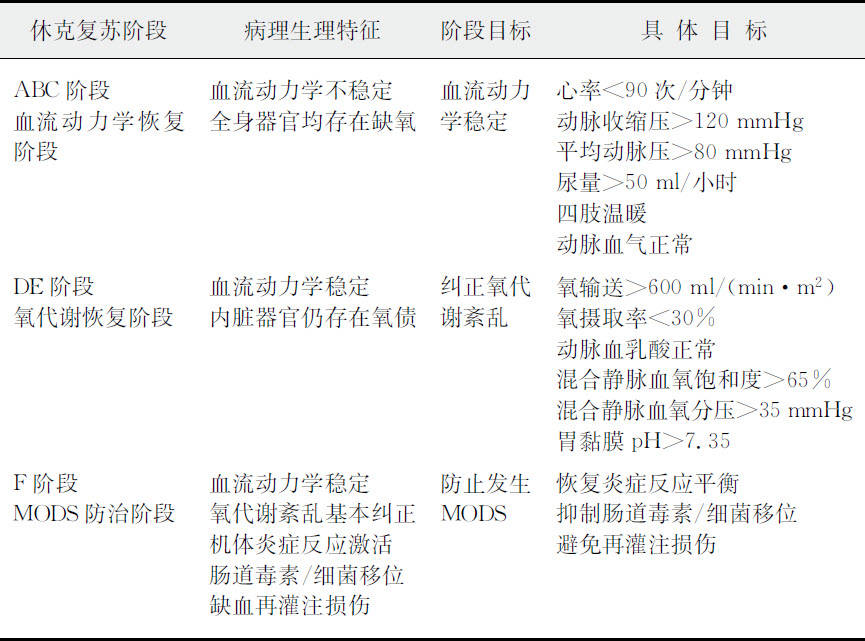
\includegraphics[width=\textwidth,height=\textheight,keepaspectratio]{./images/Image00020.jpg}
\end{table}

\subsection{感染性休克的复苏}

\subsubsection{对感染性休克患者怎么选择合适的液体进行复苏?}

复苏液体包括晶体液和天然或人工合成的胶体液。严重感染和感染性休克时液体复苏采用胶体还是晶体一直存在争议。对感染患者和外科术后患者晶体液和胶体液复苏的临床荟萃分析显示,尽管晶体液复苏所需的液体量明显高于胶体液,但胶体液和晶体液复苏对肺水肿发生率、住院时间和28天病死率均无明显影响。针对16个重症医学科近7000例危重患者进行研究,发现两组机械通气时间和肾脏替代治疗时间均无显著性差异,28天病死率也无明显差异。且针对合并颅脑创伤的患者进行亚组分析,白蛋白组的病死率明显高于生理盐水组。然而,最近的研究显示使用白蛋白进行复苏具有器官保护的作用,因此2012年《重症感染和感染性休克治疗指南》中提议在重症感染及感染性休克的早期液体复苏组合中加入白蛋白。

与晶体液相比,分子量大的人工胶体溶液在血管内的滞留时间长,扩容效果可能优于晶体。然而研究显示人工胶体与晶体进行复苏对病死率无明显影响,而人工胶体甚至有一定的肾损伤作用。Bayer等针对重症感染的患者比较羟乙基淀粉及生理盐水的效果,研究发现羟乙基淀粉组尽管在开始两天内需要的液体量较少,但急性肾损伤的发生率明显增高,两组病死率无明显差异。最近发表在新英格兰医学杂志的研究
\protect\hyperlink{text00008.htmlux5cux23ch12-7}{\textsuperscript{{[}12{]}}}
显示,与晶体液相比,针对重症感染及感染性休克的患者使用羟乙基淀粉进行复苏增加90天病死率,并且增加肾脏替代治疗的比例。2012年最新的《重症感染和感染性休克治疗指南》推荐早期使用晶体进行液体复苏,并建议不用分子量>200Da和(或)取代基>0.4的羟乙基淀粉。

\subsubsection{感染性休克患者应以什么速度进行液体复苏?}

对于疑有低容量状态的严重感染患者,应行快速补液试验,即在30分钟内输入500~1000ml晶体液或300~500ml胶体液,同时根据患者反应性(血压升高和尿量增加)和耐受性(血管内容量负荷过多)来决定是否再次给予快速补液试验。新的指南推荐对于重症感染导致的组织低灌注的患者,初始液体复苏以输注晶体液≥1000ml开始,最初4~6小时内至少输注30ml/kg的液体量,而对于部分患者可能需要更快和更大的输液量。

快速补液试验也称为容量负荷试验,是快速纠正低血容量状态的最佳方法。快速补液试验明显不同于持续静脉液体输入,通过短时间内输注大量的液体,密切观察血压、心率、尿量、肢体温度等反映器官灌注的指标,同时需要严密观察肺部湿啰音等肺水肿的征象,以评价机体对快速补液的耐受性。因此,快速补液试验能够评估患者对容量负荷的反应,评价血容量减少的程度,从而指导液体治疗。静脉血管扩张和毛细血管通透性增加是严重感染和感染性休克重要的病理生理特征。静脉血管的扩张使容量血管的容积明显增加,毛细血管通透性增加使大量的血管内液体渗漏到血管外组织间隙和第三间隙,使有效循环血量急剧降低。因此,在严重感染和感染性休克早期,往往需大容量的液体复苏,每日的液体输入量远高于出量(即正平衡)。

当然,由于不同感染性休克患者有效循环血量降低的程度不同,不同患者液体正平衡的程度就有很大差异,因此,液体平衡量并不能说明液体复苏是否充分。

\subsubsection{何谓早期目标导向治疗?}

早期目标导向治疗(early goal-directed
therapy,EGDT)是指一旦临床诊断为严重感染,应尽快进行积极液体复苏,6小时内达到以下复苏目标:①中心静脉压8~12mm
Hg;②平均动脉压≥65mm
Hg;③每小时尿量≥0.5ml/kg;④中心静脉或混合静脉血氧饱和度≥70%。早期目标导向治疗可明显降低严重感染和感染性休克患者的病死率
\protect\hyperlink{text00008.htmlux5cux23ch13-7}{\textsuperscript{{[}13{]}}}
\textsuperscript{,}
\protect\hyperlink{text00008.htmlux5cux23ch14-7}{\textsuperscript{{[}14{]}}}
。Rivers等组织的一项随机、对照、单中心的严重感染早期目标性复苏治疗研究表明,若能在严重感染发生6小时内实现复苏目标,严重感染的28天病死率能从49.2%降低到33.3%,60天的病死率从56.9%降低到44.3%
\protect\hyperlink{text00008.htmlux5cux23ch13-7}{\textsuperscript{{[}13{]}}}
。提示对严重感染和感染性休克早期实施目标导向治疗具有重要的临床意义。早期目标导向治疗以中心静脉血氧饱和度或混合静脉血氧饱和度≥70%为目标。机械通气和腹高压可导致患者胸腔内压增高,使中心静脉压升高,因此对于机械通气和腹高压的患者,可以将中心静脉压12~15mm
Hg作为复苏目标。

若液体复苏后中心静脉压达8~12mm
Hg,而中心静脉血氧饱和度或混合静脉血氧饱和度仍未达到70%,需输注浓缩红细胞使血细胞比容达到30%以上,或输注多巴酚丁胺(最大剂量至每分钟20μg/kg)以达到复苏目标。

对于重症感染和感染性休克患者,实现治疗目标的步骤,首先应给予初始的容量复苏,而如果低血压对于初始容量复苏无反应,则迅速加用缩血管药以维持血压≥65mmHg。在容量复苏后仍然存在持续低血压或者初始的血乳酸水平>4mmol/L,则需要液体复苏使中心静脉压≥8mmHg;监测中心静脉血氧饱和度或混合静脉血氧饱和度,若未达到70%,则应根据血红蛋白浓度,输注浓缩红细胞使血细胞比容达到0.30以上;若中心静脉血氧饱和度或混合静脉血氧饱和度仍未达到70%,应给予多巴酚丁胺(最大剂量至每分钟20μg/kg)以达到复苏目标。

\subsubsection{何谓容量反应性?}

容量反应性指心脏对静脉输液的反应。容量有反应定义为通过输注500ml晶体,心输出量可以增加10%以上。当患者处于心功能曲线的上升段时,输液可以明显增加心输出量,增加氧输送,改善组织灌注;当处于心功能曲线平台段时,输液不能明显增加心输出量,不能改善组织灌注,反而增加左心舒张末期压力,加重肺水肿。研究显示,重症患者仅有约50%的患者有容量反应。因此,对于需要进行液体复苏的患者,正确评价患者的容量反应性至关重要。

\subsubsection{何时需要进行容量反应性的评估?}

当患者出现急性体液血液丢失或存在严重的感染等情况,如果出现有效循环血量不足的表现,如低血压、心率增快、尿量减少、皮肤湿冷、花斑和意识改变等,则提示患者需要输液补充有效循环血量,此时应该评估患者的容量反应性,明确患者对补液治疗的耐受性,明确患者是否可以通过补液增加有效循环血量,以改善组织灌注,从而从补液治疗中获益。

\subsubsection{评价容量反应性的方法有哪些?}

研究发现经过输液之后,反映心脏前负荷的指标如中心静脉压、肺动脉嵌顿压、左心舒张末期容积等值的变化不能有效反映容量反应性。目前的容量反应性的评估方法为通过改变心脏的前负荷来观察每搏输出量或心输出量的变化。

常用的评价容量反应性的方法包括:

(1)快速补液试验 静脉输注500ml晶体,比较输液前后心输出量的变化,如果输液后心输出量增加>10%,则定义为患者容量有反应。

(2)被动抬腿试验 通过抬高患者的双下肢,可以使得双下肢的血液回流至心脏,增加心脏前负荷。有研究证实被动抬腿试验可以使回心血量增加300~400ml。具体方法为:基础体位为45°的半卧位,然后改为平卧位并抬高双下肢至45°,维持至少1分钟(图\ref{fig2-3})。如果被动抬腿后心输出量增加10%以上,定义为容量有反应。

\begin{figure}[!htbp]
 \centering
 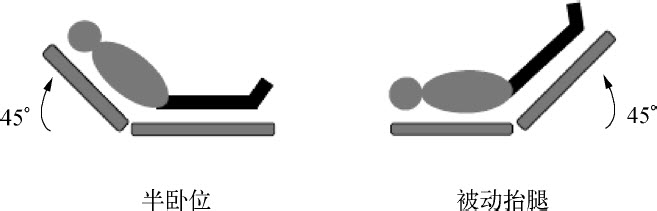
\includegraphics{./images/Image00021.jpg}
 \captionsetup{justification=centering}
 \caption{被动抬腿试验体位模式图}
 \label{fig2-3}
  \end{figure} 

(3)下腔静脉变异度 随着呼吸运动,胸腔压力的改变将引起回心血量的改变,下腔静脉的直径相应出现改变。下腔静脉直径在吸呼气间的改变称为下腔静脉变异度。当容量不足时,由于吸气引起的回心血量增加会引起下腔静脉直径明显缩小。研究证实,当患者机械通气、无明显自主吸气努力时,下腔变异度>18%定义为容量有反应;而当患者存在自主吸气努力时,下腔静脉变异度>50%提示为容量有反应。

\subsubsection{糖皮质激素在感染性休克中如何使用?}

许多学者致力于研究糖皮质激素对严重感染及感染性休克的作用。既往研究表明,大剂量糖皮质激素治疗感染性休克增加病死率、二重感染率以及消化道出血发生率,从而提示大剂量糖皮质激素治疗感染性休克是有害的。临床不应推荐大剂量糖皮质激素治疗感染性休克
\protect\hyperlink{text00008.htmlux5cux23ch15-7}{\textsuperscript{{[}15{]}}}
。

之后的一些研究显示,应激剂量糖皮质激素可改善感染性休克患者的预后。然而,近年欧洲的一个大规模、双盲、随机对照研究显示,小剂量激素尽管能缩短低血压的时间,减少血管活性药物使用剂量,但同时也增加感染的发生率,并不能改善患者预后。Sligl等进行的荟萃分析提示,使用小剂量激素不能改善患者预后。因此,2012年《重症感染和感染性休克治疗指南》推荐,如果液体复苏以及使用血管活性药物后血流动力学能够趋于稳定,建议不使用激素治疗。仅当在液体复苏及使用血管活性药物血流动力学仍然不稳定,才使用激素治疗。推荐应用氢化可的松,最大剂量200mg/天。

\subsubsection{感染性休克患者使用激素治疗前需要做促肾上腺皮质激素刺激试验吗?}

重症患者往往存在肾上腺皮质功能相对不全。有研究显示,对促肾上腺皮质激素刺激有反应(使用促肾上腺皮质激素30~60分钟后,皮质醇水平增加>9μg/dl)的患者,使用应激剂量的激素可以改善预后。然而,其他研究均未得出类似的结果。最近的研究显示,不管促肾上腺皮质激素刺激有反应还是无反应,应激剂量激素治疗均不改善患者预后。因此,2012年《重症感染和感染性休克治疗指南》建议使用激素前不需行促肾上腺皮质激素刺激试验。

\subsubsection{何谓严重感染的集束化治疗?}

血流动力学紊乱是严重感染和感染性休克最突出的表现。血流动力学的支持是感染性休克重要的循环支持手段,目的是改善血流动力学状态、改善器官灌注,逆转器官功能损害。早期的目标指导性治疗已经证实明显改善感染性休克患者的预后。除了血流动力学管理,还有其他一些重要治疗也显示出明显改善预后的效果。

为了规范临床严重感染及感染性休克的治疗行为,最终达到降低病死率的目的,除了积极有效的血流动力学支持外,还需要同时联合其他有效的治疗,也就是形成一个联合治疗的套餐,是为“感染的集束化治疗”(sepsis
bundle)。集束化治疗的目的一方面为了促进临床医生联合应用重症感染和感染性休克的各项治疗措施,规范临床医生的治疗行为;另一方面也是为了提高各项治疗措施的可行性和依从性,最后达到改善预后的目的。

早期的集束化治疗是指在确诊严重感染和感染性休克后立即开始并在6小时内必须完成的治疗措施,包括血清乳酸水平测定;抗生素使用前留取病原学标本;急诊在3小时内、重症医学科在1小时内开始广谱的抗生素治疗;如果有低血压或血乳酸>4mmol/L,立即给予液体复苏(20ml/kg),如低血压不能纠正,加用血管活性药物,维持平均动脉血压≥65mmHg;持续低血压或血乳酸>4mmol/L,液体复苏使中心静脉压≥8mmHg,中心静脉血氧饱和度≥70%。血流动力学监测和治疗是早期集束化治疗中最重要的组成部分,早期集束化治疗强调时间紧迫性,尽可能在1~2小时内放置中心静脉导管,监测中心静脉压和中心静脉血氧饱和度,开始积极液体复苏,6小时内达到上述目标,并通过监测和调整治疗维持血流动力学的稳定。确诊严重感染和感染性休克的早期6小时又被称为“黄金6小时”,显示出早期集束化治疗在临床上的重要性。

尽早达到集束化治疗的目标,可以明显改善严重感染和感染性休克患者的预后。Rivers的研究显示,6小时内实施并完成目标导向的血流动力学治疗可以显著降低病死率。英国的另一项前瞻性、双中心的研究显示,101例严重感染和感染性休克患者纳入观察,在6小时内达到感染的集束化治疗复苏目标组病死率为23%,而6小时内未达标组病死率为49%,也就是达标组病死率下降2倍。可见,尽早达到6小时集束化治疗目标可以显著降低严重感染和感染性休克患者病死率,在临床上应积极推行。

之前推荐的24小时集束化的治疗内容包括严格控制血糖,使用小剂量糖皮质激素,采用肺保护性通气测率以及使用小剂量活化蛋白C,除了肺保护性通气策略外,其余治疗内容均未被证实有效,甚至被证实为增加患者病死率。因此,新的《重症感染和感染性休克治疗指南》已经取消了24小时集束化治疗。

\subsection{心源性休克的治疗}

\subsubsection{心包填塞的特征是什么,怎样进行紧急救治?}

心包腔是指壁层心包与心脏表面的脏层心包之间的空隙。正常心包腔内有少量淡黄色液体润滑着心脏表面。由于心包的弹力有限,急性心包积血或积液达150ml即可限制血液向心脏回流和心脏跳动,引起急性循环衰竭,甚至可引起心跳骤停。心包填塞可引起心脏收缩和舒张受限,是导致梗阻性休克最常见的原因。血流动力学特征是右房压、右室舒张末期压、肺动脉舒张压均明显升高,但肺动脉嵌顿压不高,同时心输出量明显降低。床边超声心动图检查可见心包积液、右房和右室舒张受限、吸气时室间隔左移。吸气时,由于室间隔左移,减少左室舒张期充盈,同时胸腔内压降低,使左心后负荷增加,导致心输出量降低,脉搏变细,形成“奇脉”,这也是心包填塞的特征性表现之一。

急性心包填塞一旦出现,必须争分夺秒地进行抢救治疗。当胸壁锐器伤和胸部挤压伤患者出现进行性血压下降、面色苍白、心率增快、心音遥远、颈静脉怒张、烦躁不安时,应首先考虑急性心包填塞,应紧急做心包穿刺,排血减压、缓解填塞,暂时改善血液动力学,争取抢救时间,并在输血补液纠正失血性休克同时准备紧急开胸手术探查,严格麻醉管理,严防心脏骤停,补充足够的血液,术中清除心包腔积血,恢复心脏正常收缩和舒张功能,精细准确地修补心脏破损处。术后严密监测心功能。

\subsubsection{心源性休克的治疗包括哪些内容?}

心源性休克与其他类型休克的血流动力学特征有所不同,常表现为前后负荷过高,而心输出量减少,导致有效循环血量不足。治疗原则为调整心脏前、后负荷,改善心肌收缩和舒张功能,以达到纠正休克的目的。

(1)一般性治疗 减少搬动患者,采取上半身抬高15°体位,有利于肺部通气(因膈肌下移),同时下肢下垂,减少静脉回流,减低心脏前负荷,另外,应进行生命体征严密的监测。

(2)建立畅通的气道 若患者的自主呼吸力量足够,立即给予鼻导管或面罩给氧,使动脉血氧分压>70mmHg,动脉血二氧化碳分压<45mmHg。如果患者一般情况不稳定,有意识障碍、动脉血氧分压低或出现明显的肺水肿,应立即气管插管并给予机械通气治疗,以保证氧供,并减轻心脏负担。

(3)建立确切的静脉通道 可放置颈内静脉、锁骨下静脉导管,既可提供快速输液的静脉通道,又可获得可靠的血流动力学指标。

(4)镇静和止痛 应用镇静剂和止痛剂来解除患者紧张、焦虑,缓解由于创伤、手术引起的疼痛,可以应用吗啡或芬太尼。

(5)血管活性药物的应用 由于心源性休克的患者心肌收缩力下降、外周血管阻力明显增加,可常规应用血管活性药物。酸中毒使心肌和血管系统对血管活性药物不敏感,故应在纠正酸中毒的基础上给予血管活性药物。

多巴胺与多巴酚丁胺:常规用药剂量为每分钟2~20μg/kg。多巴胺小剂量(小于每分钟5~10μg/kg)作用于多巴胺受体和β受体,大剂量时主要作用于α受体。多巴酚丁胺为单纯的β受体激动剂,具有增加心率、增加心输出量、增加肾血流量的作用。对于有右心功能不全或肺动脉高压者,多巴酚丁胺可以降低肺动脉血管阻力。

肾上腺素:常用剂量为每分钟0.01~0.2μg/kg,可以增加心输出量,还可解除支气管平滑肌痉挛。

硝普钠和硝酸甘油:若患者外周血管痉挛明显或应用上述药物剂量过大引起α受体作用过强,可应用这两种药物来改善外周血管痉挛。硝普钠的常用剂量为每分钟0.1~5μg/kg,硝酸甘油为每分钟0.1~2μg/kg。另外,应用扩血管药物可减轻心脏的前后负荷,减轻左心室舒张末压力,使左心功能改善。

洋地黄类药物:应用时应慎重。可引起严重心律失常,也可因肝肾代谢障碍出现洋地黄中毒。但心率快、血钾浓度正常时,可小剂量应用。

氨力农与米力农:是一种非洋地黄类、非儿茶酚胺类的强心药,并有扩张外周血管的作用,可减轻心脏的前后负荷。氨力农的用量为每分钟6~10μg/kg,米力农为每分钟0.25~1μg/kg。

(6)保护心肌药物的应用 可以应用极化液或能量合剂、辅酶Q10、护心通等心肌保护药物。

\subsubsection{心源性休克需要心脏辅助装置或外科治疗吗?}

部分心源性休克在药物治疗无效情况下需要外科治疗,另有部分心源性休克必须进行外科治疗。

当心源性休克积极地用药物治疗(如应用正性肌力药物)效果不明显或无效时,没有必要一味增加正性肌力药物的剂量而错失治疗的机会,此时应考虑使用心脏辅助循环装置。这些装置有主动脉内球囊反搏(intra-aortic
balloon counterpulsasion
therapy,IABP)、体外膜氧合、左心转流、右心转流和左、右心转流。心源性休克患者,当心脏指数每分钟<2L/m\textsuperscript{2}
、中心静脉压>15mmHg、左房压>20mmHg时,应果断地放置主动脉内球囊反搏。

部分心源性休克必须用外科手术治疗,如急性心脏损伤后心肌出血造成心包填塞、二尖瓣腱索断裂、急性心肌缺血造成心肌梗死且在16小时之内、心肌梗死后室间隔穿孔、经皮冠状动脉球囊成形术介入治疗时造成急性血流动力学不稳定等。由于这些原因引起的心源性休克药物治疗无效,应积极采用心脏辅助装置或外科方法予以治疗。

\subsubsection{什么是心脏手术后低心排综合征?}

心脏手术后低心排综合征是心脏手术后出现的心源性休克,是心脏术后严重并发症,发生率为2%~10%,常常在术后4~6小时发生,其主要原因是左心室功能障碍,与术前心功能障碍、手术过程、术后的缺血再灌注损伤、术后的心肌缺血等因素有关,表现为持续的低心输出量和左心室充盈压增高。术后心肌梗死也是术后低心排的一个重要原因,其发生率约为5%。

\subsubsection{心脏术后低心排综合征怎么处理?}

在心脏术后低心排综合征诊断成立后,应建立合理的治疗方案,类似于心肌梗死后心源性休克的治疗。首先是保证充分的氧供、氧合及维持理想的心率和心律,并仔细评估左心室的充盈压。可以将输血输液的速度加快到左心室充盈压允许的耐受限,如果心输出量在这些初始措施干预后仍维持在危险的低水平,应积极应用血管活性药物。最常用的药物为多巴胺、多巴酚丁胺、肾上腺素、氨力农、米力农等,必要时可应用扩血管药物(如硝普钠)来降低心脏前后负荷。

手术后发生低心排综合征时,超大剂量使用正性肌力药物,往往弊大于利。强烈的α受体作用会使周围血管和内脏血管强烈收缩,导致严重的组织和器官灌注不足,产生难以逆转的严重酸中毒,患者最后可因低心排综合征、严重酸中毒、多器官功能障碍综合征而死亡。

若对药物治疗无效,或是在手术结束后无法脱离体外循环机,应积极地考虑对衰竭的心脏进行机械辅助治疗。这些患者大部分(60%~80%)在应用主动脉内球囊反搏以后即可恢复,仅有很少一部分患者(0.2%~1%)需要进一步的机械辅助循环装置(如左心辅助装置)。

心脏术后主动脉内球囊反搏的适应证是手术结束时无法脱离体外循环机、术后低心排综合征、术后出现顽固性室性心律失常等。

\subsection{感染性休克血管活性药物的选择和应用}

\subsubsection{如何把握感染性休克血管活性药物应用指征?}

应用血管活性药物是感染性休克重要的循环支持手段,目的是改善血流动力学状态、恢复组织器官灌注、逆转器官功能损害
\protect\hyperlink{text00008.htmlux5cux23ch16-7}{\textsuperscript{{[}16{]}}}
。有效循环血量不足是感染性休克的基本问题,血容量恢复正常或前负荷基本恢复是血管活性药物应用的前提。一般认为,血管活性药物的应用指征是经积极液体复苏,而平均动脉压仍然低于65mmHg。然而,当感染性休克出现威胁生命的低血压时,在积极液体复苏的同时,往往需要早期应用血管活性药物,以维持重要脏器的灌注
\protect\hyperlink{text00008.htmlux5cux23ch17-7}{\textsuperscript{{[}17{]}}}
\textsuperscript{,}
\protect\hyperlink{text00008.htmlux5cux23ch18-7}{\textsuperscript{{[}18{]}}}
。

\subsubsection{感染性休克患者应用血管活性药物的目的是什么?}

血管活性药物的应用目的主要包括:

(1)提高血压是感染性休克时应用血管活性药物的首要目标 儿茶酚胺类、血管加压素类药物大多具有血管收缩作用,能够实现提高血压的目的。

(2)改善内脏器官灌注 内脏器官血流灌注减少是休克的主要病理生理特点,即使休克患者的血压被纠正,内脏器官依然可能缺氧,可能导致多器官功能障碍综合征。

因此,改善器官组织灌注,特别是内脏器官灌注,逆转组织缺血才是休克复苏和血管活性药物应用的关键。对休克血管活性药物疗效的评价就不应单纯以升高血压为标准,而应关注器官灌注是否改善。

\subsubsection{理想的血管活性药物应具备什么样的作用?}

基于血管活性药物应用的目的是改善器官组织灌注,特别是内脏器官灌注,以逆转组织缺血,因此理想的血管活性药物应符合:①迅速提高血压,改善心脏和脑血流灌注;②改善或增加肾脏和肠道等内脏器官的血流灌注,纠正组织缺氧,防止多器官功能障碍综合征。血管活性药物的选择必须考虑其对内脏灌注的影响。在存在心肌抑制或既往存在心功能不全的患者可选择或加用有正性肌力作用的血管活性药物。

\subsubsection{多巴胺的作用特点是什么?}

多巴胺是儿茶酚胺类药物之一,在体内是合成肾上腺素的前体物质。对α、β和多巴胺受体均具有兴奋作用,其效应具有剂量依赖性。每分钟1~5μg/kg主要激动多巴胺受体DA\textsubscript{1}
和DA\textsubscript{2}
,使肾脏、肠系膜、冠脉血管扩张,增加肾血流量和钠的排出;每分钟5~10μg/kg主要激动β受体,表现为心脏正性肌力作用,增加心肌收缩力和心率。多巴胺每分钟1~10μg/kg同时对肠道和肾脏等内脏血管表现为多巴胺受体样效应。当剂量达到每分钟10~20μg/kg时,主要作用于α受体,表现为缩血管效应。但各剂量在危重患者的作用常重叠,应密切观察多巴胺的剂量效应关系。

多巴胺的这种剂量效应特点对临床应用有着明显的影响。从多巴胺对心脏的作用中可以发现,多巴胺通过增加心输出量和扩张冠状动脉增加冠状动脉的血流量,改善心肌的灌注,然而,多巴胺的剂量增大后,β\textsubscript{1}
受体兴奋导致心肌做功增加,氧耗量增大,反而使心肌的氧供需平衡的失调更为加重,所以,在应用多巴胺时,一定要根据患者的具体情况,精确地调整剂量,决不能只把多巴胺当成所谓的“升压药”来使用。大剂量多巴胺的主要副作用是强烈的心脏兴奋和心律失常。当多巴胺剂量高于每分钟20μg/kg,应更换其他药物。如患者外周血管阻力显著降低,可应用去甲肾上腺素;而外周血管阻力明显增高,则可使用肾上腺素。

\subsubsection{如何评价去甲肾上腺素在感染性休克治疗中的地位?}

去甲肾上腺素是肾上腺素能神经末梢释放的递质,对α受体有很强的兴奋作用,对β受体也具有一定的激动作用,表现为强烈的血管收缩和一定的正性肌力作用,使全身小动脉和小静脉均收缩,外周阻力增加,血压升高,增加冠状动脉和脑动脉的血流量,增加心室做功。

去甲肾上腺素在休克治疗中曾经是一个非常有争议的血管活性药物。以往认为,去甲肾上腺素可引起严重的血管痉挛,导致器官灌注减少,最终导致器官功能衰竭。但近来的研究显示,在感染性休克治疗中,去甲肾上腺素并不引起内脏组织的缺血,在与多巴胺的比较中,去甲肾上腺素不会引起内脏血流灌注减少,反而有助于恢复组织氧供需平衡。感染性休克患者外周血管阻力降低,应用去甲肾上腺素可明显提高血压,在保证心脏和脑等重要器官灌注的同时,能改善内脏血流灌注。近年的5个随机对照研究比较了多巴胺与去甲肾上腺素治疗感染性休克的疗效,研究证实去甲肾上腺素有降低病死率的趋势。因此,2012年《重症感染和感染性休克治疗指南》推荐将去甲肾上腺素作为感染性休克患者的首选升压药。

去甲肾上腺素必须由中心静脉导管给药。如外周静脉输注,一旦渗漏皮下,可能引起皮肤组织坏死。

\subsubsection{多巴胺和去甲肾上腺素在休克治疗中究竟谁更有优势?}

多巴胺和去甲肾上腺素是休克治疗中最常用的血管活性药物,但究竟哪种药物在休克治疗中更具有优势,一直没有明确的答案。以往在充分液体复苏后患者仍不能达到目标血压时,往往使用多巴胺来提升血压。新英格兰医学杂志在2010年3月发表了一篇针对多巴胺和去甲肾上腺素在休克治疗中比较的多中心、随机、对照研究\textsuperscript{{[}20{]}}
。这项研究共纳入1679名需要血管活性药物维持血压的休克患者,依照随机、双盲原则,其中858名患者使用多巴胺,821名使用去甲肾上腺素。结果显示,在主要终点事件28天的死亡率上,两者无明显差异。但是在并发症中,多巴胺组心律失常的发生率要明显高于去甲肾上腺组。在亚组分析中,感染性休克亚组和低血容量性休克亚组,多巴胺和去甲肾上腺素组两者28天死亡率无明显差异,但在心源性休克亚组,多巴胺组死亡率要高于去甲肾上腺素组。因此多巴胺在休克治疗特别是心源性休克治疗中的安全性问题值得我们关注。而对于感染性休克患者,仅在心律失常发生的风险非常低并且心功能明显受损(心功能Ⅳ级)或心率较慢的情况下使用多巴胺。

\subsubsection{肾上腺素的作用机制是什么?}

肾上腺素对α和β受体均具有强烈兴奋作用,主要表现心肌收缩力增加,心率加快,心肌氧耗增加,皮肤、黏膜及内脏小血管收缩,但冠状动脉和骨骼肌血管扩张。不同剂量肾上腺素对心血管受体可产生不同的效应:小剂量(每分钟0.01~0.05μg/kg)主要激动β\textsubscript{1}
及β\textsubscript{2}
受体,增加心肌收缩力和心输出量,扩张周围血管,而α受体效应不明显;剂量增加到每分钟0.1μg/kg时,除β效应外,α效应明显;当剂量每分钟0.1μg/kg时,明显激动α受体,同时表现出强烈收缩周围血管作用,易导致心动过速和心律失常。

感染性休克患者出现以下情况时,可考虑使用肾上腺素:①去甲肾上腺素无效;②血流动力学表现为低心输出量和低外周血管阻力。

在心脏术后患者存在严重低心输出量时,可单独使用或与其他血管活性药物联合使用。

\subsubsection{多巴酚丁胺在何时选择应用?}

多巴酚丁胺为强烈的β受体激动剂,具有强烈的β\textsubscript{1}
受体和一定的β\textsubscript{2}
、α受体兴奋作用。能增加心肌收缩力,提高心输出量,加快心率,并可能增加心肌氧耗。但对心率和心肌氧耗的影响明显低于异丙肾上腺素。多巴酚丁胺对外周血管不表现出明显的直接作用,可能是因为多巴酚丁胺对血管的作用较弱,而且同时兴奋外周血管β受体和α受体,其对血管的舒缩效应相抵所致。

多巴酚丁胺可增加每搏输出量、心输出量,作用强度与应用剂量成正相关,心肌收缩力和心输出量增加的同时使外周阻力有所下降,这更有利于心肌氧供需平衡的维持和心脏功能的恢复。多巴酚丁胺是心源性休克的常用血管活性药物,当感染性休克患者出现低心输出量时,也可应用多巴酚丁胺。

应用多巴酚丁胺时应从小剂量每分钟2μg/kg开始,根据病情变化及使用效果调整剂量,剂量高于每分钟10μg/kg时可引起心率增快,甚至心律失常。多巴酚丁胺也可导致心律失常,但发生率较异丙肾上腺素和多巴胺低。

\subsubsection{血管加压素在感染性休克治疗中有何地位?}

血管加压素是休克时一种重要的内源性应激激素,休克患者常常存在血管加压素不足和血管加压素受体数量下调。血管加压素主要通过下列机制恢复血管紧张性,收缩血管、提高血压:①激活血管加压素V\textsubscript{1}
受体;②下调血管平滑肌ATP敏感的钾通道的活性;③减少诱导型一氧化氮的合成;④与去甲肾上腺素等血管活性药物有协同作用。因此,血管加压素能有效升高平均动脉压和每搏输出量指数,降低心率、中心静脉压、平均肺动脉压及其他血管活性药的需要量,并特异性表现为收缩出球小动脉效应大于收缩入球小动脉效应,增加肾小球灌注压而增加肾小球滤过压,增加尿量,改善肾功能,但有可能导致血液在肠壁内分流及肠道氧需增加,可能加重胃肠黏膜缺氧。

一项观察血管加压素联合去甲肾上腺素与单纯使用去甲肾上腺素在感染性休克患者28天死亡率和90天死亡率的多中心、随机、双盲对照研究结果显示:两组间总体的28天死亡率和90天死亡率无明显差异,总体不良事件发生率也无明显差异。亚组比较中,仅在感染性休克程度较轻的患者(去甲肾上腺素用量≤15μg/分钟),血管加压素组28天和90天死亡率均较去甲肾上腺素组低;而在严重感染性休克患者(去甲肾上腺素用量≥15μg/分钟),两组28天死亡率无明显差异。

对于伴有急性肾衰竭的感染性休克的患者,2009年的一项研究显示:与单纯使用去甲肾上腺素比较,血管加压素联合去甲肾上腺素不但可以减缓肾衰竭的进展,而且显著减少了28天死亡率和90天死亡率。

在联合应用血管加压素的剂量问题方面,2010的一项研究结果显示:在感染、全身炎症反应或心脏手术后的需要去甲肾上腺素>0.6μg/kg·分钟维持的血管扩张性休克的患者,应用血管加压素0.067U/分钟较0.033U/分钟能使去甲肾上腺素的用量更少,而且血管加压素的剂量与去甲肾上腺素的用量及改善心血管功能的有效性方面均有显著的相关性。

可见,对于程度较轻的感染性休克患者和合并急性肾功能不全的感染性休克患者,小剂量血管加压素与去甲肾上腺素联合使用可获益。而在使用剂量方面,0.067U/分钟会比0.033U/分钟效果更佳。

\subsubsection{小剂量的多巴胺具有肾脏保护作用吗?}

传统认为,小剂量多巴胺具有选择性扩张肾血管、降低肾血管阻力和增加尿量的作用,被称为肾脏剂量多巴胺。但近来研究证实多巴胺的肾脏保护作用并不确切。在动物试验和志愿者中,小剂量多巴胺仅仅是通过抑制近曲小管钠的重吸收而促进钠的排出,具有增加尿量作用。

(1)心衰患者的研究 1964年,Goldberg
\protect\hyperlink{text00008.htmlux5cux23ch16-7}{\textsuperscript{{[}16{]}}}
以6例充血性心衰患者为研究对象,观察小剂量多巴胺的肾脏效应,结果每分钟1.3~3.6μg/kg多巴胺不增加心输出量时,对肾脏无保护作用;若心输出量增加,尿量也明显增加。可以推测肾脏剂量多巴胺增加尿量是心输出量增加的结果,而不是多巴胺对肾脏的直接效应。

(2)围手术期应用研究 通过观察小剂量多巴胺(每分钟3μg/kg)对肝移植、主动脉手术、阻塞性黄疸术后患者肾脏功能影响证实,小剂量多巴胺对术后患者的肾脏功能并无保护作用,不增加肾小球滤过率,也不降低急性肾衰竭患者的患病率。

(3)感染性休克的应用研究 严重感染患者应用小剂量多巴胺,虽通过抑制近曲小管钠的重吸收促进钠的排出,具有利尿作用,但并不增加肌酐清除率,对急性肾衰竭无预防作用。

(4)急性肾衰竭患者的应用研究 小剂量多巴胺并不能降低急性肾衰竭患者的病死率,也不能降低急性肾衰竭患者需要血液透析治疗的比例。大规模的随机对照临床研究也显示,328位早期肾功能障碍的危重患者应用小剂量多巴胺和安慰剂对危重患者血肌酐峰浓度、肾脏替代治疗的时间、尿量、肾功能恢复时间均无明显影响,重症医学科生存率、最终生存率、重症医学科住院时间、总住院时间、心律失常发生率差异亦无显著性。

可见,小剂量多巴胺无肾脏保护作用,危重病患者不推荐常规应用多巴胺进行肾脏保护。

\subsubsection{去甲肾上腺素对感染性休克患者肾功能有何影响?}

以往认为,去甲肾上腺素可引起严重的肾血管痉挛,导致急性肾衰竭。这主要源于Girbes的报道,他用去甲肾上腺素诱导出动物急性肾衰竭,但其应用剂量很大,而且是动脉内直接给药。实际上,目前尚无去甲肾上腺素导致急性肾衰竭的临床研究报道。近年来研究证实,在感染性休克中,去甲肾上腺素对肾脏功能具有保护作用。

去甲肾上腺素可导致健康志愿者肾血管收缩,肾脏血浆流量减少,但肾脏血管阻力无明显增加,尿钠排泄分数和肾小球滤过率均无明显改变。

去甲肾上腺素对感染性休克患者的肾脏功能具有保护作用:前瞻随机双盲对照试验观察每分钟0.5~5μg/kg去甲肾上腺素与每分钟2.5~25μg/kg多巴胺对感染性休克患者血流动力学和尿量的影响,结果显示多巴胺组仅31%(5/16)达到预定的治疗目标(灌注恢复,并持续6小时),而去甲肾上腺素组93%(15/16)达到治疗目标,而且该组患者尿量明显增加。多巴胺组中血流动力学改善不明显的11例患者,改用去甲肾上腺素10例有效。可见,去甲肾上腺素可改善感染性休克患者血流动力学状态,并明显增加患者尿量,改善肾脏功能。

因此,去甲肾上腺素不仅改善感染性休克患者血流动力学状态,而且能够改善肾功能。

\subsubsection{多巴酚丁胺和肾上腺素对危重病患者肾脏功能有影响吗?}

多巴酚丁胺对危重病患者的肾脏功能具有保护作用。Duke等选择肾脏功能轻度受损的危重患者25例,分别应用200μg/分钟多巴胺或175μg/分钟多巴酚丁胺静脉注射5小时,结果多巴酚丁胺组血压和心输出量较高,尿量和尿钠排泄分数无明显增加,但肌酐清除率明显增加。而多巴胺组尿量增加,肌酐清除率无明显改变。可见,多巴酚丁胺明显优于多巴胺,可改善肾脏灌注,提高肾小球滤过率。至于多巴酚丁胺改善肾脏功能的机制,可能与增加心输出量,改善肾脏灌注有关;是否具有直接肾脏效应尚待进一步研究。

肾上腺素是强大的α受体和β受体激动剂。休克患者应用肾上腺素,可提高心输出量和血压,增加氧输送。但肾上腺素可能加重肾脏损害,使用应慎重。

肾上腺素可增加严重感染动物和患者的肾脏血流量,但是同时导致肾小球滤过率明显降低,加重肾脏损害。Bersten
\protect\hyperlink{text00008.htmlux5cux23ch17-7}{\textsuperscript{{[}17{]}}}
以正常绵羊和腹腔感染绵羊为研究对象,首先发现正常动物和感染动物对肾上腺素具有不同的反应性。正常绵羊应用肾上腺素后,肾动脉血流量显著增加50%,肾血管阻力显著降低,而应用多巴胺后,肾动脉血流仅增加25%。对于严重感染动物,肾上腺素可使动物肾血流增加25%,而多巴胺使肾动脉血流仅增加15%。两药对正常动物的作用明显强于感染动物。进一步观察对肾脏功能的影响,结果正常动物应用肾上腺素后,肌酐清除率无显著改变,而感染动物应用肾上腺素后,肌酐清除率首先显著降低,之后有所上升,呈现双相改变。可见,肾上腺素应用可能加重肾脏功能损害。

\subsubsection{多巴胺能够改善肠道等内脏器官灌注吗?}

一般认为,肠道血管具有多巴胺受体,多巴胺具有扩张肠道血管,增加肠道血流灌注的作用。但目前研究表明,尽管多巴胺能够增加肠道血流量,但肠道血管分流增加,黏膜血流反而减少,导致肠道缺血加重。

(1)多巴胺明显增加肠道血流量 动物实验及健康志愿者的研究均显示,小剂量多巴胺能够扩张肠系膜动脉,增加肠系膜动脉血流量。

(2)多巴胺明显加重肠道缺血 胃肠道黏膜pH值是反映胃肠道缺血缺氧的敏感指标。Marik观察10例感染性休克患者,应用多巴胺后,平均动脉压、心输出量、氧输送和氧耗均明显增加,但胃肠道黏膜pH值明显降低,说明感染性休克患者应用多巴胺后,血压升高的同时,肠道缺血缺氧明显加重。

尽管多巴胺明显增加血压、心输出量,明显增加胃肠道血流量和氧输送,但同时增加了全身氧耗、胃肠道血液分流和肠黏膜氧耗量,最终可能导致肠道缺氧加重。

\subsubsection{多巴酚丁胺对内脏器官血流和灌注有何影响?}

多巴酚丁胺为强烈的β受体激动剂,通过兴奋β\textsubscript{1}
受体增加心输出量和氧输送,改善肠道灌注,β\textsubscript{2}
受体激动则导致肠道内的血流重分布,改善肠道缺氧,降低氧耗,使胃肠道黏膜pH升高。Joly等研究了14例感染性休克的患者,给予每分钟7.5μg/kg多巴酚丁胺,发现多巴酚丁胺明显增加心输出量,增加肠道血流,改善胃黏膜灌注。感染性休克患者的全身氧输送和胃肠道黏膜pH值随多巴酚丁胺剂量增加(每分钟0~10μg/kg)而升高,呈剂量依赖性关系。目前认为,多巴酚丁胺增加全身氧输送时,同比例增加肠道的氧输送,同时多巴酚丁胺使肠道内的血流重分布,血流从肠壁向肠黏膜重分布,增加胃肠黏膜灌注,改善胃肠道黏膜氧供需平衡。

\subsubsection{为什么去甲肾上腺素是感染性休克一线的血管活性药?}

以往认为,去甲肾上腺素是强烈的α受体兴奋剂,具有强烈缩血管作用,增加心脏后负荷,降低心输出量,同时也导致内脏血管收缩,加重内脏器官缺血,因此,以往去甲肾上腺素很少用于感染性休克的治疗。最近的研究结果与传统观念形成鲜明对比,感染性休克患者应用去甲肾上腺素,可明显改善全身血流动力学,改善肠道等内脏器官的缺血缺氧,明显优于多巴胺、肾上腺素等血管活性药物。

(1)心输出量并不降低 提高外周血管阻力,导致心输出量下降,是应用去甲肾上腺素的顾虑之一。感染性休克具有外周血管阻力明显降低的特征,决定了应用去甲肾上腺素后,心输出量不会明显降低。感染动物应用去甲肾上腺素后,不仅不会引起心输出量降低,部分动物心输出量轻度增加。心输出量增加可能与去甲肾上腺素兴奋β受体,使心肌收缩力增加,冠状动脉灌注增加有关,也可能与血压升高,间接改善心脏灌注有关。

(2)增加肠道血流量和氧输送 去甲肾上腺素不仅明显提高全身氧输送,还明显增加肠道等内脏器官的血流量和氧输送。内毒素休克动物的研究显示,去甲肾上腺素能够改善内毒素引起的外周血管强烈扩张,增加全身和内脏器官的氧输送。临床研究也提示在不增加全身氧输送的情况下,去甲肾上腺素能够明显逆转感染性休克患者外周血管扩张,改善胃肠道血流灌注。

(3)改善肠道缺氧 研究显示去甲肾上腺素明显提高感染性休克患者的平均动脉压、心输出量、全身氧输送,同时胃肠道黏膜pH值显著升高。可见,感染性休克患者应用去甲肾上腺素能够改善肠道缺血。

(4)去甲肾上腺素对感染性休克患者的肠道黏膜屏障具有保护作用 Sautner等采用猪内毒素休克模型,观察去甲肾上腺素对动物回肠、结肠黏膜完整性的影响,结果去甲肾上腺素对回肠和结肠黏膜无损伤作用,而且不会引起细菌移位。

总之,应用去甲肾上腺素不仅能迅速改善感染性休克患者的血流动力学状态,而且能够改善胃肠道等内脏器官缺血,临床研究也证实去甲肾上腺素治疗感染性休克疗效确切,被推荐为治疗感染性休克的首选药物。

\subsubsection{联合应用去甲肾上腺素和多巴酚丁胺的时机和效果如何?}

去甲肾上腺素能够迅速改善感染性休克患者的血流动力学状态,迅速提高血压,改善心脏和脑血流灌注,改善或增加肾脏和肠道等内脏器官的血流灌注,减轻胃肠道等内脏器官缺血,恢复氧供需平衡。在合并心肌抑制、心功能不全或心源性休克的患者可联合使用去甲肾上腺素和多巴酚丁胺,改善心脏功能,增加心输出量,改善组织灌注。

去甲肾上腺素与多巴酚丁胺联合应用可进一步改善肠道缺氧,感染性休克患者联合应用去甲肾上腺素和小剂量多巴酚丁胺后,胃肠道的血流量明显增加,肠道血流量的增加幅度不仅高于单用去甲肾上腺素,而且也高于肾上腺素。同时去甲肾上腺素与多巴酚丁胺联合应用也明显降低动脉血乳酸水平,提高胃肠黏膜pH值,降低胃黏膜与动脉血二氧化碳分压差。周韶霞等
\protect\hyperlink{text00008.htmlux5cux23ch18-7}{\textsuperscript{{[}18{]}}}
的研究也证实了这一结论。

另外,去甲肾上腺素和多巴酚丁胺的产热效应均明显低于肾上腺素,联合应用去甲肾上腺素和多巴酚丁胺不会增加全身和肠道的氧耗。

因此,去甲肾上腺素是有效治疗感染性休克的血管活性药物,可提高血压,改善组织灌注。在合并心功能障碍时可联合应用多巴酚丁胺。

\subsubsection{如何评价肾上腺素在感染性休克治疗中的地位?}

肾上腺素具有强大的正性肌力作用,明显增加休克患者心率、心输出量和氧输送,也明显增加肠道血流量和氧输送,但同时更大幅度地增加肠道氧耗,结果导致肠道缺氧明显加重,增加胃肠黏膜pH值。

(1)加重全身缺氧 健康志愿者应用肾上腺素后,全身氧耗明显增加,糖分解利用增加,导致血糖和乳酸水平明显上升。提示肾上腺素增加健康志愿者氧耗,导致代谢紊乱和组织缺氧加重。

动脉血乳酸升高可由组织缺氧引起,也可能是丙酮酸脱氢酶功能降低,乳酸代谢障碍(如肝脏功能损害)的结果。研究证实,乳酸/丙酮酸比例<10,提示乳酸堆积是由于乳酸代谢障碍所致,而比例>10则提示乳酸堆积是组织缺氧引起乏氧酵解、乳酸产生过多的结果。因此,测定乳酸/丙酮酸比例可判断乳酸升高的原因。

肾上腺素引起的乳酸升高是组织缺血缺氧的结果,而不是乳酸代谢障碍的结果。Levy观察了感染性休克患者应用肾上腺素后动脉血乳酸和乳酸/丙酮酸比例的变化。结果显示肾上腺素应用1小时后,动脉血乳酸明显升高,而且乳酸/丙酮酸>10,并持续12小时。提示感染性休克患者应用肾上腺素,可加重全身缺氧和乳酸酸中毒。肾上腺素是所有儿茶酚胺药物中产热效应最严重的药物,应用肾上腺素后明显增加机体氧耗,可能是肾上腺素引起或加重全身缺氧及乳酸酸中毒的重要原因。严重感染和感染性休克患者应用肾上腺素后,可导致全身性的缺血缺氧加重。

(2)加重肠道缺氧 感染性休克患者应用肾上腺素后,尽管肠系膜血流量明显增加,却反而使肠道缺血加重。其机制与肠道氧供氧需失衡有关。肾上腺素增加肠道氧需的程度,远远超过了肾上腺素导致肠道氧输送的增加,其净效应是肠道氧供氧需失衡,肠道缺血缺氧加重。

(3)损害肠道屏障 肾上腺素可严重损害感染性休克动物的肠道屏障功能。Sautner等采用猪的内毒素休克模型,观察肾上腺素对动物肠黏膜pH值和回肠、结肠黏膜的影响,结果肾上腺素不仅导致肠黏膜pH值明显降低,而且也引起动物回肠和结肠黏膜损害。说明肾上腺素明显降低肠道灌注,并损害肠黏膜完整性。

尽管上述结果提示肾上腺素可能有害,但是目前缺乏循证医学证据表明肾上腺素会增加感染性休克患者的病死率。有4项随机对照研究比较了肾上腺素和去甲肾上腺素治疗感染性休克的作用,结果显示两者疗效并无显著差异。目前指南推荐当去甲肾上腺素不能维持血压需要加用其他血管活性药物时,可以加用肾上腺素。

\subsection{心源性休克血管活性药物的选择和应用}

\subsubsection{心源性休克血管活性药物应用指征是什么?}

低心排综合征或心源性休克是临床常见的、最严重的循环衰竭,常见于心血管大手术后、冠心病及严重感染性休克的患者。血管活性药物是重要的循环支持措施。当心肌收缩功能受到损害或抑制出现低心排综合征时,通过积极调整前负荷,使左室舒张末压或左房压达到正常范围甚至高限,积极调整和改善心肌舒张功能后,若心输出量和氧输送仍未达到合适水平,具有应用正性肌力药物的指征。

\subsubsection{常用的心源性休克血管活性药物作用机制是什么?}

低心排综合征或心源性休克是临床常见的、最严重的循环衰竭。常见于心血管大手术后、冠心病及严重感染性休克的患者。血管活性药物是重要的循环支持措施。

常用的血管活性药物分为:①肾上腺素能激动剂;②洋地黄类药物;③磷酸二酯酶抑制剂;④钙增敏剂;⑤血管扩张药物如硝普钠、硝酸甘油等。钙增敏剂是近年来应用于临床的一种新型正性肌力药物。

肾上腺素能激动剂的作用机制如表\ref{tab2-5}。\footnote{* α受体兴奋:皮肤、黏膜血管及内脏血管收缩;β\textsubscript{1}
受体兴奋:心肌收缩力增强,心率加快,心肌耗氧量增加;β\textsubscript{2}
受体兴奋:冠状动脉和骨骼血管扩张;多巴胺受体兴奋:尿量增加。}

\begin{table}[htbp]
\centering
\caption{常用肾上腺素能血管活性药物的作用机制比较\textsuperscript{*}}
\label{tab2-5}
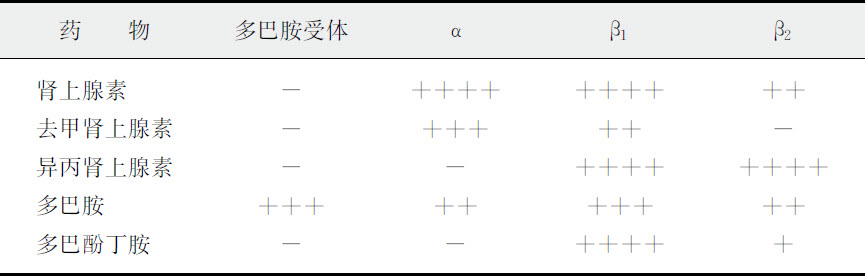
\includegraphics[width=\textwidth,height=\textheight,keepaspectratio]{./images/Image00022.jpg}
\end{table}



\subsubsection{洋地黄类药物作用机制和在休克中的地位如何?}

洋地黄类药物具有正性肌力、负性传导和负性频率效应。抑制心力衰竭心肌细胞膜上的Na\textsuperscript{+}
-K\textsuperscript{+} -ATP酶,使细胞内Na\textsuperscript{+}
水平升高,促进Na\textsuperscript{+} -Ca\textsuperscript{2+}
交换,使细胞内Ca\textsuperscript{2+}
水平提高,从而发挥正性肌力作用。另外,洋地黄还抑制了副交感传入神经的Na\textsuperscript{+}
-K\textsuperscript{+}
-ATP酶,提高了位于左室、左房和右房入口处及主动脉弓和颈动脉窦的压力感受器的敏感性,抑制性传入冲动的数量增加,进而使中枢神经系统下达的交感兴奋性减弱。

洋地黄类药物多用于慢性心力衰竭和某些心律失常的治疗。增强心肌收缩力的同时不收缩血管,心率不加快。伴快速房颤时,还能控制心室率。大多数洋地黄类药物的起效时间长,作用持续时间长,治疗剂量和中毒剂量接近。增强心肌收缩力作用比肾上腺素和多巴酚丁胺弱。

休克是一种急性循环衰竭,尤其是在合并多个器官功能受累时病情的发展变化往往很快,因此,休克治疗中,一般应用起效迅速、安全可靠、半衰期短、剂量容易掌握的药物如儿茶酚胺类药物多巴胺、多巴酚丁胺、去甲肾上腺素等。但并不是说在休克的治疗中不能使用洋地黄类药物,洋地黄主要用于心源性休克或合并慢性心功能不全或快速房颤时。

\subsubsection{心源性休克可以使用去甲肾上腺素吗?}

去甲肾上腺素是以激动α受体为主的儿茶酚胺类药物,主要起收缩外周血管的作用。由于心源性休克的血流动力学以低排高阻为特点,因此既往不主张使用去甲肾上腺素来治疗心源性休克,避免外周阻力进一步增高,增加心脏后负荷,2007年美国心脏协会《指南》也推荐心源性休克的首选药物为多巴胺。然而,2010年在新英格兰医学杂志上发表的一个随机对照研究发现,对所有的休克患者而言,相比多巴胺,去甲肾上腺素不增加患者病死率,并且能减少心律失常的发生。有意思的是,在亚组分析中,针对心源性休克患者,去甲肾上腺素组较多巴胺组明显降低病死率,从而提示在心源性休克中可以考虑使用去甲肾上腺素。

\subsubsection{磷酸二酯酶Ⅲ抑制剂作用机制是什么?怎样临床应用?}

磷酸二酯酶Ⅲ抑制剂是非强心苷、非儿茶酚胺类强心药,兼有正性肌力及扩血管效应,主要抑制心肌和血管平滑肌的磷酸二酯酶Ⅲ,抑制环磷酸腺苷(cAMP)的水解,从而增加心肌细胞环磷酸腺苷浓度,激活钙通道增加钙内流,增强心肌收缩功能,同时增加血管平滑肌内环磷酸腺苷浓度,使血管扩张。小剂量使用时主要表现为正性肌力作用,扩张血管作用随剂量的增加而逐渐增强。该类药物的适应证包括:准备行心脏移植以及终末期的心衰、短期用于难治性心衰、心脏术后。β受体阻滞剂治疗后出现失代偿性心衰需要强心和(或)对多巴酚丁胺反应不良时,因磷酸二酯酶Ⅲ抑制剂的作用不被β受体阻滞剂所拮抗,可选用磷酸二酯酶Ⅲ抑制剂短期使用。

临床常用的磷酸二酯酶Ⅲ抑制剂为氨力农(amrinone)和米力农。氨力农负荷量0.25~0.75mg/kg(3~5分钟),维持量每分钟1.25~10μg/kg。米力农(milrinone)是第二代磷酸二酯酶Ⅲ抑制药,血流动力学效应与氨力农类似,但正性肌力作用比氨力农强,半衰期约2.4小时,较多巴酚丁胺长得多,在肾衰竭时可能会产生蓄积,负荷量25~50μg/kg(10分钟),维持量每分钟0.25~1μg/kg。

\subsubsection{钙增敏剂的作用机制和临床适应证是什么?怎样临床应用?}

钙增敏剂是一种新型的正性肌力药物,它可以与心肌肌钙蛋白C结合,增加心肌肌钙蛋白C对Ca\textsuperscript{2+}
的敏感性,从而通过无需提高细胞内Ca\textsuperscript{2+}
浓度的方式增强心肌收缩力,且不影响心率,心肌耗氧量也未见明显增加;同时钙增敏剂还可通过使ATP敏感的K\textsuperscript{+}
通道开放而产生血管舒张作用,使得冠状动脉阻力血管和静脉容量血管舒张,从而改善冠脉的血流供应;另外它还可抑制磷酸二酯酶Ⅲ。目前钙增敏剂主要适用于传统治疗(利尿剂、血管紧张素转换酶抑制剂和洋地黄类)疗效不佳的由收缩功能不全所致的低心排患者,用药后可有心输出量和每搏输出量上升,体循环阻力和肺循环阻力的下降,使心力衰竭症状好转。

一项对有心肌抑制的严重感染患者的研究发现,与多巴酚丁胺比较,钙增敏剂具有增加心指数、增加左室射血分数、降低左室舒张末期容积、降低肺动脉楔压、增加胃黏膜血流,增加尿量和降低血乳酸浓度的作用,能更好地增强心肌收缩力和改善组织灌注。为临床脓毒症心肌抑制和正性肌力药物的使用提供了新的思路。

目前临床主要使用的钙增敏剂是左西孟旦,治疗的初始负荷剂量为6~12μg/kg,时间应>10分钟,之后应持续输注每分钟0.1μg/kg。对于同时应用血管扩张剂或(和)正性肌力药物的患者,治疗初期的推荐负荷剂量为6μg/kg。在负荷剂量给药时以及持续给药开始30~60分钟内,密切观察患者的反应,如反应过度(低血压、心动过速),应将输注速率减至每分钟0.05μg/kg或停止给药。如初始剂量耐受性好且需要增强血液动力学效应,则输注速率可增至每分钟0.2μg/kg,持续给药时间通常为24小时。在左西孟旦停药后,未发现有耐药和反弹现象。血液动力学效应至少可持续24小时,停药后,此效应可能持续9天。

\subsubsection{静脉应用硝普钠时应注意哪些问题?}

硝普钠是一种有效的血管扩张剂,可同时扩张小动脉和小静脉,有效降低心脏的前负荷和后负荷,减轻肺水肿,减少心肌的耗氧量。因此,硝普钠可有效降低血压,对心力衰竭也有较好的治疗作用。

硝普钠的特点是起效快,作用效果强,作用持续时间短,非常符合危重患者的治疗要求。临床应用时需严格控制硝普钠的剂量,同时在血流动力学监测下进行。硝普钠扩血管作用强,稍有剂量波动也可能导致血流动力学的大幅度改变。在注射硝普钠的静脉通路上如果有其他液体,这些液体的输入速度也可能影响硝普钠的输入速度,从而影响硝普钠的作用效果,甚至导致病情的突然改变,临床应加以充分注意。

硝普钠在体内代谢产生硫氰化物,如持续大剂量使用超过3天则可能引起血中硫氰化物的蓄积,导致硫氰酸盐中毒,但临床上并不常见。硝普钠见光分解,使用时要注意避光输注。

\subsubsection{硝酸甘油有哪些特点?临床应用应注意哪些问题?}

硝酸甘油以扩张静脉为主,对冠状动脉有扩张作用,大剂量时对静脉和动脉都有扩张作用。静脉应用具有起效快、作用时间短、效果确实可靠等特点,尤其是对冠状动脉的扩张作用,使硝酸甘油在对合并有心肌供血不足的危重病人中起到非常重要的作用。在心力衰竭或心源性休克的治疗中,硝酸甘油可以降低心脏的前负荷,还可以稍降低后负荷。因此,在改善心肌做功状态的同时,硝酸甘油扩张冠状动脉,增加了心肌的血液供应,改善了心肌的氧供需平衡。

硝酸甘油应小剂量持续静脉泵入,一般由1~5μg/分钟开始,逐渐增加剂量以达到最佳的血流动力学效应。

近年来人们对硝酸甘油的耐受性有了更多的认识,一般认为,持续静脉应用硝酸甘油时间过长,机体可产生耐受性,不宜大剂量长期使用。

\subsection{主动脉内球囊反搏在休克的应用}

\subsubsection{什么是体外反搏?}

体外反搏1962年开始于美国,是一种无创的体外辅助循环装置,其原理是通过对人体臀部及下肢与心脏周期同步的无创性序贯加压,将血流驱回至上半身,增加心脏、脑、肾等重要脏器的舒张期血液灌流。体外反搏利用包裹在人体下肢的气囊,在心脏舒张期对人体施加外压,将其下肢以及臀部的血液驱回主动脉,从而增加心肌的灌注压和供血(增加30%~50%),达到改善血管功能、改善血液循环及代谢等目的,使心脏供氧增加、心肌损耗减少,它能降低血液黏稠度,改善微循环,减少血小板聚集,降低血栓素水平,是治疗心脑血管疾病的一种无创伤疗法。

心脏的射血是正向搏动,是心收缩期血液流动的动力泵(第一泵);而体外反搏是心舒张期反向搏动,是心舒张期驱动血液流动的动力泵(第二泵)。体外反搏治疗把外在气体动力作用于人体循环系统,把气体的动力转化为人体血液循环的动力,一方面加速人体血液循环的速度,在动脉系统,由一个心跳周期单脉传递(第一泵),转变为一个周期的双脉传递(第一泵+第二泵),这样既加速血流传递,增加血管内血液流动的切应力,又增加血管舒/缩运动的频率(增加1倍血管舒缩运动,无需像运动那样增加心率、增加耗氧来实现,有助于硬化血管弹性的维护和恢复),对于静脉系统,由下半身静脉无动力或弱动力的回流,变为由第二泵挤压所致的有动力搏动性静脉向心回流,增加回心血量,从而增加心输出量(30%左右);另一方面,体外反搏治疗介入循环系统,改变原有的收缩期灌注压高,舒张期灌注压低的循环灌注模式,变为收缩期灌注压降低,舒张期灌注压明显增加,这种灌注模式最大的受益者是心脏,可使得心脏冠脉在舒张期灌注量增加40%左右,收缩期血流灌注下降5%,总灌注量增加30%~50%。大脑血流灌注不受收缩期和舒张期的影响,体外反搏治疗可增加颈动脉舒张期血流量的30%左右,而收缩期血流灌注量则下降10%左右,总血流灌注量增加20%~30%,这种增加不需要增加心脏的动力,是体外反搏作用的结果。再者,体外反搏促进血液循环加速,势必加速全身微循环血流,有助于微循环障碍的改善。

\subsubsection{何谓主动脉内球囊反搏,其工作原理是什么?}

主动脉内球囊反搏是机械性辅助循环方法之一,是一种通过物理作用,提高主动脉内舒张压,增加冠状动脉供血和改善心脏功能的治疗方法,通过对血流动力学的影响而对心功能障碍起辅助性治疗作用。早期,主动脉内球囊反搏主要用于冠状动脉供血不足及心脏手术围手术期的辅助性治疗。随着主动脉内球囊反搏技术的不断完善和临床应用的发展,现已广泛应用于心功能不全危重病患者的抢救和治疗。

主动脉内球囊反搏是将一个带有球囊的导管置入患者主动脉内,球囊位于降主动脉的近心端,导管尖端位于左锁骨下动脉开口以下。根据患者自主心率或动脉压力,触发主动脉内球囊反搏的驱动装置,使球囊在心室舒张期充盈,心室收缩开始前快速排空。球囊在心脏舒张期充盈,把主动脉内的部分血液推向主动脉根部,从而使冠状动脉的灌注压明显升高,脑的舒张期灌注压也明显升高。与此同时,球囊把一部分血液推向主动脉远端,增加了内脏器官的舒张期血流灌注,尤其是肾脏灌注。在心脏收缩前球囊突然排空,使主动脉内的压力骤然下降,左心室的射血阻力明显降低,导致心肌做功降低,氧耗量明显减少。

实验表明:主动脉内球囊反搏可使冠脉血流增加7%~50%;心室射血阻力减少46%;心输出量提高10%~40%。总之,主动脉内球囊反搏可增加心肌氧供,减少心肌氧耗,从而使心肌氧供与氧耗平衡,同时改善全身的氧代谢。

\subsubsection{主动脉内球囊反搏有哪些适应证?}

主动脉内球囊反搏主要用于心源性休克和严重低心排综合征的预防和治疗。应尽早使用,如患者出现多器官功能障碍综合征,则疗效较差。

(1)心脏内科 ①各种原因导致的心源性休克,如急性心肌梗死、左心室壁瘤、乳头肌断裂及功能不全、二尖瓣关闭不全、心肌炎或心肌病等;②不稳定性心绞痛,包括内科治疗无效的不稳定性心绞痛、变异性心绞痛持续24小时、心肌缺血致顽固性快速室性心律失常;③充血性心力衰竭;④心导管操作期间或操作后的循环支持;⑤心脏骤停的复苏。

(2)心脏外科 ①等待冠状动脉搭桥术的不稳定性心绞痛或急性心肌梗死;②心脏术前血流动力学不稳定;③心脏手术中的心源性休克;④心脏手术后难以脱离体外循环;⑤术后发生心源性休克或心功能衰竭;⑥心脏移植术前后。

(3)其他 ①其他类型的休克合并心功能不全;②患严重心脏病需行非心脏手术;③特殊情况下暂时辅助增加脑血流。

\subsubsection{主动脉内球囊反搏有禁忌证吗?}

主动脉内球囊反搏的禁忌证包括绝对和相对禁忌证:

(1)绝对禁忌证 ①严重主动脉关闭不全;②胸、腹主动脉瘤;③影响导管插入的外周动脉疾病。

(2)相对禁忌证 ①终末期心脏病;②不可逆转的脑损害;③主动脉、髂动脉严重病变或感染;④出血性疾病;⑤转移性恶性肿瘤。

\subsubsection{主动脉内球囊反搏可产生哪些血流动力学效应?}

主动脉内球囊反搏所产生的血流动力学效应主要包括以下5个方面。

(1)舒张早期压力升高 辅助后舒张早期动脉压力明显升高,一般高于动脉收缩压,明显增加心脏、脑和内脏器官的舒张期灌注。

(2)舒张末期压力降低 辅助后的舒张末期动脉压力降低,一般低于原动脉舒张压,使左心室的射血阻力降低,后负荷下降,左心室收缩末容积减少,降低心肌氧耗。

(3)辅助后的收缩压降低 由于球囊在心室收缩前突然排空,使主动脉内的压力骤然下降,而且低于原舒张压,导致左心室后负荷明显降低,使辅助之后的收缩压略低于原收缩压,进一步降低室壁张力,降低心肌氧耗。

(4)冠状动脉灌注增加 舒张期动脉压力明显升高是冠状动脉灌注改善的主要原因。心室后负荷降低,心室收缩末期容积减少,导致心室舒张期压力降低,也可部分增加冠状动脉灌注。

(5)心输出量增加 由于左心室后负荷明显降低,降低了左心射血阻力,使心输出量增加。另外,心脏灌注改善,也可使心功能逐渐改善,心输出量逐渐增加。

\subsubsection{怎样选择合适的主动脉内球囊反搏导管?}

主动脉内球囊反搏导管有单球囊导管和双球囊导管两种,但目前多使用单球囊导管。导管由高分子材料聚氨酯构成,壁薄透明,柔软而成纺锤形。

选择合适的导管很重要。不合适的导管不仅达不到治疗效果,还可造成动脉损伤及血细胞破坏。成人导管球囊充盈时,应占主动脉直径的75%~90%。气囊容积应大于每搏量的50%。一般根据身高选择:身高>180cm,应选用球囊容积50ml的导管;身高165~180cm,可选用球囊容积40ml的导管;身高<165cm,可选球囊容积30ml的导管。

\subsubsection{怎样置入主动脉内球囊反搏导管?}

导管置入方式包括切开法和穿刺法两种。

(1)穿刺法 又称Seldinger法。按常规消毒、铺巾、局部麻醉后,穿刺股动脉,通过穿刺针芯将导引钢丝置入动脉,退出穿刺针。沿导引钢丝扩张血管,置入导管鞘。球囊导管接单向阀,注射器抽尽囊内气体。沿导引钢丝将球囊导管置入,导管尖端插至主动脉左锁骨下动脉开口下2cm处。

床边操作时,置管前应先初步测量需置入导管的深度(一般为股动脉至胸骨角)。操作结束后X线检查,确定导管尖端不超过第4胸椎水平。若在床边X线指导下操作,可直接放置到合适位置或造影确认位置。

操作后注意固定导管鞘和导管,以防滑出。最后将导管接反搏泵。

(2)切开法 手术分离出股动脉,直视下插入导管。适用于穿刺困难的病例如休克、股动脉硬化者、股动脉触摸困难者或体外循环术中。由于需手术植入,操作费时,出血和感染的机会多,且停用后还要行动脉修补术,现在多被穿刺法取代,只在穿刺法失败后才用。

\subsubsection{主动脉内球囊反搏需要抗凝吗?}

由于目前球囊材料较好,抗凝要求并不严格。一般采用低分子右旋糖酐10ml/小时持续静脉点滴,即可达到防止血栓形成的目的。当然,也可仅用阿司匹林抗凝。

对于高凝状态的患者,应用肝素抗凝,25~50mg静脉注射后,按5~15U/分钟持续静脉泵入,使部分凝血活酶时间延长1倍。

\subsubsection{怎样调节主动脉内球囊反搏泵?}

(1)监测心电图 一般采用心电图触发,选择R波高尖、T波低平的导联。

(2)监测主动脉压及压力波形 动脉压力波形包括升支、降支和重搏波。

(3)选择反搏触发方式 一般采用心电图R波触发,获得大而可靠的R波是关键,心律失常时也可用动脉波触发,甚至使用固有频率反搏。

(4)调整反搏时相 球囊充气应调节在主动脉瓣关闭时,因动脉波形传播有所延迟,触发应在主动脉重搏波切迹前40~50毫秒开始,主动脉收缩压的下降支与反搏波的上升支形成巨大的“V”波,这是球囊充气时间正确的典型波形;球囊排气应调节在主动脉瓣即将开放前,以减少左心后负荷(图\ref{fig2-4})。心电图上,球囊充气于T波降支,放气常于R波或R波稍前。

\begin{figure}[!htbp]
 \centering
 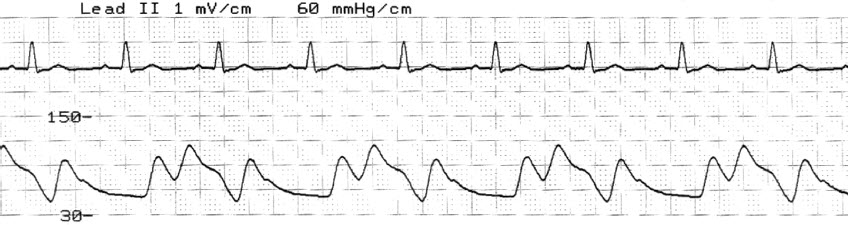
\includegraphics{./images/Image00023.jpg}
 \captionsetup{justification=centering}
 \caption{正常主动脉压和主动脉内球囊反搏波形(1∶2反搏)}
 \label{fig2-4}
  \end{figure} 

(5)选择反搏频率 根据患者心率和所需辅助强度进行选择。开始治疗时,若心率<100次/分,反搏频率选择1∶1;心率>100次/分,反搏频率选择1∶2,甚至1∶3。停用过程中,逐渐降低反搏频率。

(6)反搏强度 最低不能小于最大反搏的50%。

\subsubsection{主动脉内球囊反搏充气过早或过迟的危害是什么?}

主动脉内球囊反搏必须获得满意的舒张期增压。舒张压波形较收缩压波形高,舒张末期压较无反搏时下降10~15mmHg。应注意避免以下情况:

(1)充气过早 主动脉内球囊反搏治疗时球囊充气早于主动脉关闭切迹。表现为舒张期增压波紧跟收缩波出现或舒张期增压波介入收缩波,难以鉴别(图\ref{fig2-5})。充气过早,正值心脏的射血期,射血阻力明显增加,可导致心脏后负荷明显增加,心肌氧耗增加,同时导致主动脉瓣提前关闭,增加了左室舒张末期压和肺动脉嵌顿压,导致舒张期左室室壁张力升高,冠状动脉灌注减少。

\begin{figure}[!htbp]
 \centering
 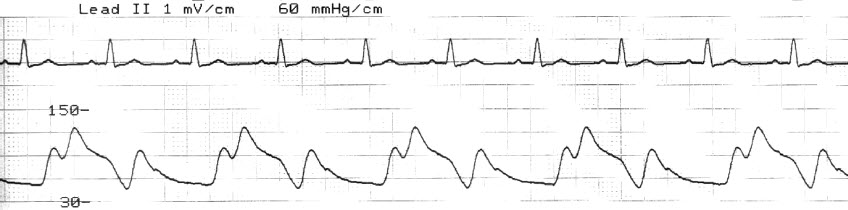
\includegraphics{./images/Image00024.jpg}
 \captionsetup{justification=centering}
 \caption{主动脉内球囊反搏球囊充气过早(1∶2反搏)}
 \label{fig2-5}
  \end{figure} 

(2)充气过迟 主动脉内球囊反搏治疗时,球囊扩张于主动脉瓣关闭切迹之后。表现为舒张期增压波出现在重搏切迹之后,尖锐的V波不存在(图\ref{fig2-6})。球囊充气过晚,主动脉内压力和血流量均已有所下降,球囊扩张而导致的血液回流明显降低,将不能最大限度地提高冠状动脉灌注压。

\begin{figure}[!htbp]
 \centering
 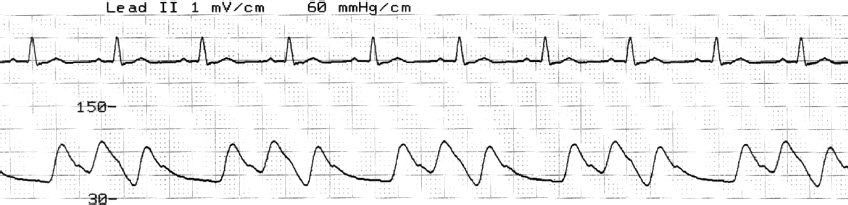
\includegraphics{./images/Image00025.jpg}
 \captionsetup{justification=centering}
 \caption{主动脉内球囊反搏球囊充气过迟(1∶2反搏)}
 \label{fig2-6}
  \end{figure} 

\subsubsection{主动脉内球囊反搏排气过早或过迟的危害是什么?}

反搏有效时,收缩压>60mmHg,脉压差>15mmHg;获得满意的舒张压增压波,辅助时舒张压升高,可>100mmHg,高于收缩压,收缩压及舒张末压下降;心肌缺血改善,心输出量增加。主动脉内球囊反搏排气过早或过迟将产生不利的影响。

(1)排气过早 主动脉内球囊反搏治疗时,球囊排空应在主动脉瓣开放之前的瞬间迅速完成,若球囊排空过早,表现为舒张期增压直线下降,增压不理想(图\ref{fig2-7})。造成主动脉内血流回流时间过短,舒张期增压降低,冠状动脉灌注改善程度较小,后负荷减少不理想,增加心肌氧耗。

\begin{figure}[!htbp]
 \centering
 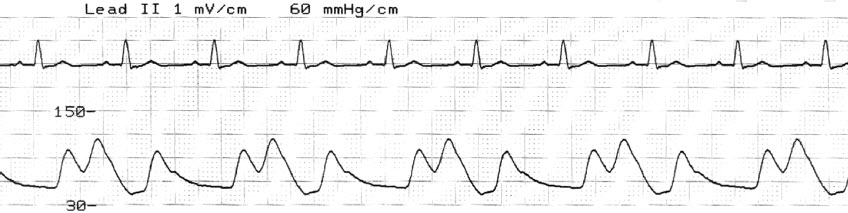
\includegraphics{./images/Image00026.jpg}
 \captionsetup{justification=centering}
 \caption{主动脉内球囊反搏球囊排气过早(1∶2反搏)}
 \label{fig2-7}
  \end{figure} 

(2)排气延迟 主动脉内球囊反搏治疗时,球囊排空过晚,造成心脏射血开始后球囊仍然阻塞在主动脉内,延长等容收缩时间,导致左心室射血阻力明显增加,心肌氧耗增加。表现为舒张期增压时间过长,波形明显增宽(图\ref{fig2-8})。

\begin{figure}[!htbp]
 \centering
 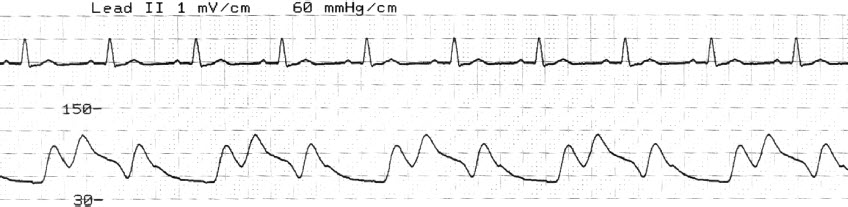
\includegraphics{./images/Image00027.jpg}
 \captionsetup{justification=centering}
 \caption{球囊排气延迟(1∶2反搏)}
 \label{fig2-8}
  \end{figure} 

\subsubsection{主动脉内球囊反搏撤机指征及应注意的事项有哪些?}

(1)撤离指标 ①生命体征逐渐平稳;②血管活性药用量减少,多巴胺每分钟<5μg/kg;③CI>每分钟2.5L/m\textsuperscript{2}
、心肌缺血改善;④平均动脉压>80mmHg、每小时尿量>1ml/kg,末梢循环良好;⑤意识清楚;⑥撤离呼吸机后血气分析指标正常;⑦减少反搏频率或强度,或停止反搏30~60分钟,上述指标稳定。

(2)撤除方法 采取两种方法撤除球囊反搏:①先减少反搏频率,由1∶1逐渐降低到1∶3;②反搏频率不变,逐渐减少球囊充气量,但充气量不得低于50%。

终止搏动后30~60分钟,必须拔出球囊导管,否则应继续反搏。拔除球囊导管后,先压迫穿刺部位远端,让血液冲出数秒,排出小血栓,然后手指移向穿刺孔压迫30分钟,直至出血完全停止。多普勒探测远端动脉,观察动脉搏动,注意是否发生动脉栓塞。

\subsubsection{主动脉内球囊反搏有哪些常见的并发症?如何处理?}

主动脉内球囊反搏并发症并不少见,可高达13.5%~36.0%。血管损伤、感染、出血为主要并发症。

(1)插管并发症 穿破动脉,导致血肿、出血;导管插入夹层;导管插入困难。操作中应选用粗细合适的导管,注意插管手法,不可粗暴操作。

(2)下肢缺血 血管痉挛、球囊导管或鞘管过粗、球囊导管或鞘管周围血栓形成、血栓脱落、下肢动脉栓塞等原因引起下肢缺血。术后应注意置管侧肢体皮温和动脉搏动。一旦出现皮肤苍白、皮温变凉、足背动脉搏动消失、肢体疼痛,需及时撤除主动脉内球囊反搏导管及导管鞘,或在对侧重新置入。如为栓子脱落,则需手术取出。上述情况应尽早处理,否则会引起下肢坏疽。

(3)感染 经皮穿刺的发生率远低于切开植入法。注意无菌操作和抗生素的应用。

(4)球囊破裂 一般由于硬物刺破所致,如粥样硬化斑块。球囊未全部退出鞘管或植入锁骨下动脉内形成折曲,折曲部位膜易被剪破裂。如出现反搏波形消失,导管内有血液吸出,应立即拔出球囊导管。否则进入球囊内的血液凝固,球囊将无法拔除。

\subsubsection{何谓左心辅助和右心辅助?有何临床意义?}

左心辅助和右心辅助是机械辅助循环的重要手段,临床常选择左心辅助,当合并严重右心功能衰竭时,可选择右心辅助或全心辅助。

1964年Spencer首次对术后病人进行左心辅助,1966年Debakey等开始用左心转流治疗不同原因引起的心源性休克,左心辅助装置的临床应用已积累了30年的经验。目前,药物治疗和主动脉内球囊反搏支持循环不能奏效时,首选左心辅助装置。

左心辅助的适应证主要有3个方面:①作为治疗性措施,使衰竭的心脏恢复功能,用于心脏手术后不能脱离体外循环机、急性心源性休克、顽固性左心衰或不易控制的致命性心律失常、心脏移植后的排斥反应、心源性休克。②作为心脏移植桥梁过渡等待供体。另外,使用方便、迅速的临时性左心辅助装置作为植入式长时间进行辅助的左心辅助装置和人工心脏的中间过渡措施,也时有报道。③作为预防性措施,主要是用于高危冠心病人做经皮冠状动脉球囊成形术,预防心跳骤停,维持动脉血压和心输出量。

经10年临床统计,使用不同类型的泵进行左心辅助时,不同病种的撤机率和长期存活率是相同的。左心辅助可使衰竭的心室卸负荷,冠状动脉窦血流、冠状动、静脉氧差和心肌氧耗分别降到正常值的47%、64%和23%。当左心辅助转流率达75%时,坏死心肌和正常心肌的交界部位心肌血流量增加;当转流率达100%时,正常心肌和交界心肌的心肌血流量均降低,但交界心肌血流量降低较少,这是心肌组织的自我调控,可改变心肌局部代谢,减少急性休克时的心肌梗死面积。左心辅助可以降低左心室舒张末期纤维长度,降低左心室做功和室壁张力,但收缩期末容量并没有改变。

长期左心辅助的心肌可发生萎缩,萎缩程度取决于转流率和持续时间,心肌细胞与间质组织的比例在辅助90天时无改变。亦有报道,完全左心室卸负荷对心脏无好处,由于完全依赖机械辅助,心肌易发生萎缩,且心室内血液淤滞,易造成血栓。

\subsubsection{怎样评价机械心脏辅助在心脏外科的应用?}

19世纪早期就有了用机械装置支持衰竭心脏的理论,到1953年心肺循环机出现后,才使这一理论在临床上得到应用。1963年,ME.DeBakey首次用机械心脏辅助装置,成功地改善了心脏手术后患者的循环和血液动力学情况,而当Cooley1969年首次将全人工心脏作为向心脏移植过渡的手段后,这一技术才逐渐得到广泛应用,至今已有大量成功的报道。近10余年来,由于心室辅助装置性能的改善,使其耐久性和生物相容性都明显提高,因而使用时间延长,使许多终末期心衰患者获得心脏移植的机会。在长期机械心脏支持过程中,不仅可以看到因心衰引起的多器官功能衰竭得到改善,而且还可以观察到心脏功能及心肌细胞损伤的恢复,部分病人在撤离机械心室辅助装置后,不需心脏移植,而保持较好的心脏功能。因而认为,心室辅助装置不只是向心脏移植过渡的桥梁,而且也是通向心肌恢复的桥梁。

目前临床上应用的循环辅助装置包括:左心室首选主动脉内球囊反搏,对程度严重的左心室衰竭可考虑左室辅助,双心室衰竭考虑双室辅助,人工心脏多用于不宜于心脏移植的病人(难以渡过排异关,要长时间等候适宜供体等)。

目前辅助循环应用于3个方面:①大面积心肌梗死引起的心源性休克;②心脏手术后严重的低心排综合征;③心脏术前过渡或因心脏功能衰竭,可能并发多脏器不同程度的功能障碍。

对急性心功能障碍、心肌损害的患者,安置心室辅助装置的目的是减少心脏做功,维持和改善全身循环,争取心肌损伤修复,如心脏手术后低心排综合征、急性大面积心肌梗死、心源性休克、急性心肌炎、心功能障碍和急性移植心脏衰竭等,这些病例若即时无供体行心脏移植,很难维持生命。心室辅助装置的置入在改善全身器官循环灌注的同时,也为心肌损伤的修复提供了时间和条件,部分病人可能在心脏功能恢复后撤离机械循环支持,文献上已有许多此类报道。国内主动脉内球囊反搏的使用在许多心脏中心已经具有丰富的临床经验。心室辅助和人工心脏还正在起步中。

\begin{center}\rule{0.5\linewidth}{\linethickness}\end{center}

参考文献

\protect\hyperlink{text00008.htmlux5cux23ch1-7-back}{{[}1{]}}
.吴在德.外科学,人民卫生出版社,第六版,2002年.

\protect\hyperlink{text00008.htmlux5cux23ch2-7-back}{{[}2{]}} .Harvey
S,Harrison DA,Singer M,et al.Assessment of the clinical
effectiveness of pulmonary artery catheters in management of patients in
intensive care(PAC - Man):a randomized controlled
trial.Lancet,2005,366:472-477.

\protect\hyperlink{text00008.htmlux5cux23ch3-7-back}{{[}3{]}} .Shah
MR,Hasselblad V,Stevenson LW,et al.Impact of the pulmonary artery
catheter in critically ill patients:meta-analysis of randomized
clinical trials.JAMA,2005,294:1664-1670.

\protect\hyperlink{text00008.htmlux5cux23ch4-7-back}{{[}4{]}}
.Mundigler G,Heinze G,Zehetgruber M,et al.Limitations of the
transpulmonary indicator dilution method for assessment of preload
changes in critically ill patients with r educed left ventricular
function.Crit Care Med,2000,28:2231-2237.

\protect\hyperlink{text00008.htmlux5cux23ch5-7-back}{{[}5{]}} .Sakka
SG,Ruhl CC,Pfeiffer UJ,et al.Assessment of cardiac preload and
extravascular lung water by single transpulmonary
thermodilution.Intensive Care Med,2000,26:180-187.

\protect\hyperlink{text00008.htmlux5cux23ch6-7-back}{{[}6{]}} .Van
Heerden PV,Baker S,Lim SI,et al.Clinical evaluation of the
non-invasive cardiac output(NICO)monitor in the intensive care
unit.Anaesth Intensive Care.2000,28:427-430.

{[}7{]}.Cholley BP,Payen D.Noninvasive techniques for measurements of
cardiac output.Curr Opin Crit Care.2005,11:424-429.

\protect\hyperlink{text00008.htmlux5cux23ch8-7-back}{{[}8{]}}
.Christine B,Bernard C.Equipment review:New techniques for cardiac
output measurement --- oesophageal Doppler,Fick principle using carbon
dioxide,and pulse contour analysis.Crit Care,2002,6:216-221.

\protect\hyperlink{text00008.htmlux5cux23ch9-7-back}{{[}9{]}}
.Dellinger RP,Carlet JM,Masur H,et al.Surviving Sepsis Campaign
guidelines for management of severe sepsis and septic shock.Intensive
Care Med,2004,30:536-555.

\protect\hyperlink{text00008.htmlux5cux23ch10-7-back}{{[}10{]}}
.Kortgen A,Niederprum P,Bauer M.Implementation of an
evidence-based“standard operating procedure”and outcome in septic
shock.Crit Care Med,2006,34:943-949.

\protect\hyperlink{text00008.htmlux5cux23ch11-7-back}{{[}11{]}} .Gao
F,Melody T,Daniels DF,et al.The impact of compliance with 6-hour and
24-hour sepsis bundles on hospital mortality in patients with severe
sepsis:a prospective observational study.Crit
Care,2005,9:R764-770.

\protect\hyperlink{text00008.htmlux5cux23ch12-7-back}{{[}12{]}} .Parner
A,Haase N,Guttormsen A,et al.Hydroxyethyl Starch 130/0.4 Versus
Ringer's Acetate in Severe Sepsis.N Engl J Med,2012,367:124-134.

\protect\hyperlink{text00008.htmlux5cux23ch13-7-back}{{[}13{]}} .Rivers
E,Nguyen B,Havstad S,et al.Early goal-directed therapy in the
treatment of severe sepsis and septic shock.N Engl J
Med,2001,345:1368-1377.

\protect\hyperlink{text00008.htmlux5cux23ch14-7-back}{{[}14{]}}
.Holthaus CV,Poirier R,Ruoff B,et al.An Administrative framework
for successfully instituting an integrated early goal-directed therapy
sepsis protocol in an emergency department.Acad Emerg
Med,2006,13:S45.

\protect\hyperlink{text00008.htmlux5cux23ch15-7-back}{{[}15{]}}
.Minneci PC,Deans KJ,Banks SM,et al.Meta-Analysis:The effect of
steroids on survival and shock during sepsis depends on the dose.Ann
Intern Med,2004,141:47-56.

\protect\hyperlink{text00008.htmlux5cux23ch16-7-back}{{[}16{]}}
.Goldberg LI,McDonald RH,Zimmerman AM.Sodium diuresis produced by
dopamine in patients with congestive heart failure.N Engl J
Med,1963,269:1060-1064.

\protect\hyperlink{text00008.htmlux5cux23ch17-7-back}{{[}17{]}}
.Bersten AD,Rutten AJ.Renovascular interaction of
epinephrine,dopamine,and intraperotoneal sepsis.Crit Care
Med,1995,23:537-544.

\protect\hyperlink{text00008.htmlux5cux23ch18-7-back}{{[}18{]}} .Zhou
SX,Qiu HB,Huang YZ,et al.Effects of
norepinephrine,epinephrine,norepinephrine-dobutamine on systemic and
gastric mucosal oxygenation in septic shock.Acta Pharmacol
Sin,2002,23:654-658.

\protect\hypertarget{text00009.html}{}{}

